\documentclass[12pt,a4paper]{book}
\usepackage{blindtext}
\usepackage{graphicx}
\usepackage{verbatim}
\usepackage{listings}
\newtheorem{lemma}{}[chapter]
\usepackage{array}
\usepackage{color}
\usepackage{hyperref}
\usepackage{amsmath}
\graphicspath{ {Images/} }
\title{Introduction to Theory of Algorithms}
\author{Yoseph Berhanu}
\date{\today}
\begin{document}
\maketitle
\tableofcontents
\part{Foundation}
\chapter{Introduction}
\section{What are Algorithms}
An \textbf{\textit{algorithm}} is an unambiguous specification of how to solve a class of problems. It is any well-defined computational procedure that takes some value or set of values as \textbf{\textit{input}} and provides some value or set of values as \textbf{\textit{output}}. Put in other words, an algorithm is a sequence of computational steps that transform an input to an output, or, a tool for solving well-specified computational problems.
\par A computer program can be viewed as an elaborate algorithm trying to explain the steps to be taken by a computer to solve a problem. The audience in computer program is a computer, hence, the algorithm is finally expressed in a language that the computer understands. We will see later on, however, that there are other 'languages' we could use in stating an algorithm depending on the audience we are trying to communicate with.
\par The concept of algorithm has existed for centuries; however, a partial formalization of what would become the modern algorithm began with attempts to solve the Entscheidungsproblem (the "decision problem") posed by David Hilbert in 1928. Subsequent formalizations were framed as attempts to define "effective calculability" or "effective method"; those formalizations included the Gödel–Herbrand–Kleene recursive functions of 1930, 1934 and 1935, Alonzo Church's lambda calculus of 1936, Emil Post's "Formulation 1" of 1936, and Alan Turing's Turing machines of 1936–7 and 1939. Giving a formal definition of algorithms, corresponding to the intuitive notion, remains a challenging problem.
\par The \textbf{problem statement/ statement of a problem} specifies the desired input/output relationship. Algorithms, therefore, describes the specifics for achieving this IO relationship. Two examples are presented here to illustrate this concept of problem statement for which students are assumed to know at least one solution algorithm.
\\

\textbf{Example 1:} Searching problem

\textbf{Input}: A sequence of n numbers $\{a_{1} , a_{2} , a_{3} ... a_{n} \}$ and a number \textit{\textbf{b}} to search for

\textbf{Output}: A index \textbf{\textit{i}} if $a_{i} = b$  or \textbf{\textit{-1}} if there exists no such  \textbf{\textit{i}} where $0 \leq i < n$ 

\textbf{Example 2}: Sorting problem

\textbf{Input}: A sequence of \textbf{\textit{n}} numbers $\{a_{1} , a_{2} , a_{3} ... a_{n} \}$

\textbf{Output}: A permutation (reordering) $\{ a_{i}, a_{ii}, a_{iii}, ..., a_{m} \}$ of the input sequence such that $\{ a_{i} \leq a_{ii} \leq a_{iii} \leq ... \leq a_{m} \}$
\\

An example input for the searching problem could be $\{93, 29, 40, 14, 26, 84\}$ and $14$, accordingly the output of a searching algorithm will be 3 (with a zero based indexing scheme). An example input sequence for the sorting problem could be {93, 29, 40, 14, 26, 84} and the output/result of a sorting algorithm for this input will be {14, 26, 29, 40, 84, 93}. Both of these inputs are called \textbf{\textit{instances}} of their respective problems.
\par
In general an instance of a problem consists of the input (satisfying whatever constraints problem statement imposes). An algorithm is said to be correct if and only if, for every input instance, it halts with the correct output. We say that a correct algorithm solves the given computational problem. 
\par
\textbf{\textit{Incorrect}} algorithms either do not halt at all or will halt with the wrong output. Incorrect algorithms might be at times useful if we can control the error rate. E.g., A \textbf{\textit{heuristic}} is a technique designed for solving a problem more quickly when classic methods are too slow, or for finding an approximate solution when classic methods fail to find any exact solution. This is achieved by trading optimal, completeness, accuracy, or precision for speed. In a way, it can be considered a shortcut.
\par
The notion of Algorithm its relationship with the notion of functions is often times confused and many use one to mean the other. However, the two notions are completely different. Function is a relation between a set of inputs and a set of permissible outputs with the property that each input is related to exactly one output. An example is the function that relates each real number \textit{x} to its square $x_{2}$. The output of a function \textit{f} corresponding to an input \textit{x} is denoted by \textit{f(x)} (read "f of x"). In this example, if the input is $ -3$, then the output is 9, and we may write $f( -3) = 9$. Likewise, if the input is 3, then the output is also 9, and we may write $f(3) = 9$. (The same output may be produced by more than one input, but each input gives only one output.) The input variable(s) are sometimes referred to as the argument(s) of the function.
\par
Algorithm on the other hand refers to the steps taken to produce the desired output. Hence, there could be more than one algorithm per function. In our previous example \textit{f(x)}, which takes in a number as an input and produces the squared value of the number as an output could be implemented in a number of ways (i.e., algorithms). One possible algorithm is to add the input value \textit{x} , \textit{x} times and return the absolute value of the sum found. Another possible implementation is to multiply the input value \textit{x} by itself once. Both of this algorithms are correct(we will define what a correct algorithm is later on), however one could be more efficient than the other. One should note that both of these assertion are valid and testable if we define the a certain computational model (discussed later)

\section{Characteristics of Algorithms}
\begin{itemize}
\item \textbf{Finiteness}: An algorithm must always terminate after a finite number of steps.
\item \textbf{Definiteness/Precision}: Each step of an algorithm must be precisely defined; the actions to be carried out must be rigorously and unambiguously specified for each case.
\item \textbf{Input} An algorithm has zero or more inputs, i.e, quantities which are given to it initially before the algorithm begins.
\item \textbf{Output}: An algorithm has one or more outputs i.e, quantities which have a specified relation to the inputs.
\item \textbf{Effectivenes}: An algorithm is also generally expected to be effective. This means that all of the operations to be performed in the algorithm must be sufficiently basic that they can in principle be done exactly and in a finite length of time.
\item \textbf{Uniqueness}: 	Results of each step are uniquely defined and only depend on the input and the result of the preceding steps.
\item \textbf{Generality}:	The algorithm applies to a set of inputs
\end{itemize}

\section{Expression of Algorithms}
\subsubsection{Flowcharts}
A flowchart is a type of diagram that represents an algorithm, work-flow or process, showing the steps as boxes of various kinds, and their order by connecting them with arrows. This diagrammatic representation illustrates a solution model to a given problem. Flowcharts are used in analyzing, designing, documenting or managing a process or program in various fields.
\subsubsection{Pseudo Code}
Pseudo Code is an informal high-level description of the operating principle of a computer program or other algorithm. It uses the structural conventions of a normal programming language, but is intended for human reading rather than machine reading. Pseudo Code typically omits details that are essential for machine understanding of the algorithm, such as variable declarations, system-specific code and some subroutines. The programming language is augmented with natural language description details, where convenient, or with compact mathematical notation. The purpose of using pseudo code is that it is easier for people to understand than conventional programming language code, and that it is an efficient and environment-independent description of the key principles of an algorithm. It is commonly used in textbooks and scientific publications that are documenting various algorithms, and also in planning of computer program development, for sketching out the structure of the program before the actual coding takes place.
\subsubsection{Programming Languages}
Since programmers can read source code of high level programming languages with ease one could use any programming language that the intended audience knows and understands.
\subsubsection{Drakon-Charts}
DRAKON is an algorithmic visual programming language developed within the Buran space project following ergonomic design principles. The language provides a uniform way to represent flowcharts of any complexity that are easy to read and understand.
\subsubsection{Control Tables}
Control tables are tables that control the control flow or play a major part in program control. There are no rigid rules about the structure or content of a control table — its qualifying attribute is its ability to direct control flow in some way through "execution" by a processor or interpreter. The design of such tables is sometimes referred to as table-driven design (although this typically refers to generating code automatically from external tables rather than direct run-time tables). In some cases, control tables can be specific implementations of finite-state-machine-based automata-based programming. If there are several hierarchical levels of control table they may behave in a manner equivalent to UML state machines
\subsubsection{In this course}
In this course we will primary use pseudo code and programming language source code to express algorithms. In both cases we will adopt a C-based language. 
\section{Classification}
There are various ways to classify algorithms, each with its own merits.
\subsection{By implementation}
\subsubsection{Recursion}
A recursive algorithm is one that invokes (makes reference to) itself repeatedly until a certain condition (also known as termination condition) matches, which is a method common to functional programming. Iterative algorithms use repetitive constructs like loops and sometimes additional data structures like stacks to solve the given problems. Some problems are naturally suited for one implementation or the other. For example, towers of Hanoi \footnote{Detailed explaniation of Tower of Hanoi is found here: \url{https://en.wikipedia.org/wiki/Tower_of_Hanoi}} is well understood using recursive implementation. Every recursive version has an equivalent (but possibly more or less complex) iterative version, and vice-versa.
\subsubsection{Logical}
An algorithm may be viewed as controlled logical deduction. This notion may be expressed as: Algorithm = logic + control.[61] The logic component expresses the axioms that may be used in the computation and the control component determines the way in which deduction is applied to the axioms. This is the basis for the logic programming paradigm. In pure logic programming languages the control component is fixed and algorithms are specified by supplying only the logic component. The appeal of this approach is the elegant semantics: a change in the axioms has a well-defined change in the algorithm.
Algorithms can be specified in English (i.e., Natural Language), as computer program, or even as a hardware design as long as it specifics precise description of the computational procedures to be followed. Most of the time we avoid using natural language for expressing algorithms due to its ambiguity, especially for complex algorithms. Instead when communicating an algorithm with other people we use one of the following \textit{'languages'}
\subsubsection{Serial, parallel or distributed}
Algorithms are usually discussed with the assumption that computers execute one instruction of an algorithm at a time. Those computers are sometimes called serial computers. An algorithm designed for such an environment is called a serial algorithm, as opposed to parallel algorithms or distributed algorithms. Parallel algorithms take advantage of computer architectures where several processors can work on a problem at the same time, whereas distributed algorithms utilize multiple machines connected with a network. Parallel or distributed algorithms divide the problem into more symmetrical or asymmetrical subproblems and collect the results back together. The resource consumption in such algorithms is not only processor cycles on each processor but also the communication overhead between the processors. Some sorting algorithms can be parallelized efficiently, but their communication overhead is expensive. Iterative algorithms are generally parallelizable. Some problems have no parallel algorithms, and are called inherently serial problems.
\subsubsection{Deterministic or non-deterministic}
Deterministic algorithms solve the problem with exact decision at every step of the algorithm whereas non-deterministic algorithms solve problems via guessing although typical guesses are made more accurate through the use of heuristics.
\subsubsection{Exact or approximate}
While many algorithms reach an exact solution, approximation algorithms seek an approximation that is closer to the true solution. Approximation can be reached by either using a deterministic or a random strategy. Such algorithms have practical value for many hard problems. One of the examples of an approximate algorithm is the Knapsack problem. The Knapsack problem is a problem where there is a set of given items. The goal of the problem is to pack the knapsack to get the maximum total value. Each item has some weight and some value. Total weight that we can carry is no more than some fixed number X. So, we must consider weights of items as well as their value.
\subsubsection{Quantum Algorithm}
They run on a realistic model of quantum computation. The term is usually used for those algorithms which seem inherently quantum, or use some essential feature of quantum computation such as quantum superposition or quantum entanglement.
\subsection{By design paradigm}
Another way of classifying algorithms is by their design methodology or paradigm. There is a certain number of paradigms, each different from the other. Furthermore, each of these categories include many different types of algorithms. Some common paradigms are:
\subsubsection{Brute-force or exhaustive search}
This is the naive method of trying every possible solution to see which is best.
\subsubsection{Divide and conquer}
A divide and conquer algorithm repeatedly reduces an instance of a problem to one or more smaller instances of the same problem (usually recursively) until the instances are small enough to solve easily. One such example of divide and conquer is merge sorting. Sorting can be done on each segment of data after dividing data into segments and sorting of entire data can be obtained in the conquer phase by merging the segments. A simpler variant of divide and conquer is called a decrease and conquer algorithm, that solves an identical subproblem and uses the solution of this subproblem to solve the bigger problem. Divide and conquer divides the problem into multiple subproblems and so the conquer stage is more complex than decrease and conquer algorithms. An example of decrease and conquer algorithm is the binary search algorithm.
\subsubsection{Search and Enumeration}
Many problems (such as playing chess) can be modeled as problems on graphs. A graph exploration algorithm specifies rules for moving around a graph and is useful for such problems. This category also includes search algorithms, branch and bound enumeration and backtracking.
\subsubsection{Randomized algorithm}
Such algorithms make some choices randomly (or pseudo-randomly). They can be very useful in finding approximate solutions for problems where finding exact solutions can be impractical (see heuristic method below). For some of these problems, it is known that the fastest approximations must involve some randomness.Whether randomized algorithms with polynomial time complexity can be the fastest algorithms for some problems is an open question known as the P versus NP problem. There are two large classes of such algorithms:
\begin{enumerate}
\item Monte Carlo algorithms return a correct answer with high-probability. E.g. RP is the subclass of these that run in polynomial time.
\item Las Vegas algorithms always return the correct answer, but their running time is only probabilistically bound, e.g. ZPP.
\end{enumerate}
\subsubsection{Reduction of Complexity}
This technique involves solving a difficult problem by transforming it into a better known problem for which we have (hopefully) asymptotically optimal algorithms. The goal is to find a reducing algorithm whose complexity is not dominated by the resulting reduced algorithm's. For example, one selection algorithm for finding the median in an unsorted list involves first sorting the list (the expensive portion) and then pulling out the middle element in the sorted list (the cheap portion). This technique is also known as transform and conquer.
\subsection{Optimization Problems}
For optimization problems there is a more specific classification of algorithms; an algorithm for such problems may fall into one or more of the general categories described above as well as into one of the following:
\subsubsection{Linear programming}
When searching for optimal solutions to a linear function bound to linear equality and inequality constraints, the constraints of the problem can be used directly in producing the optimal solutions. There are algorithms that can solve any problem in this category, such as the popular simplex algorithm. Problems that can be solved with linear programming include the maximum flow problem for directed graphs. If a problem additionally requires that one or more of the unknowns must be an integer then it is classified in integer programming. A linear programming algorithm can solve such a problem if it can be proved that all restrictions for integer values are superficial, i.e., the solutions satisfy these restrictions anyway. In the general case, a specialized algorithm or an algorithm that finds approximate solutions is used, depending on the difficulty of the problem.
\subsubsection{Dynamic programming}
When a problem shows optimal substructures – meaning the optimal solution to a problem can be constructed from optimal solutions to subproblems – and overlapping subproblems, meaning the same subproblems are used to solve many different problem instances, a quicker approach called dynamic programming avoids recomputing solutions that have already been computed. For example, Floyd–Warshall algorithm, the shortest path to a goal from a vertex in a weighted graph can be found by using the shortest path to the goal from all adjacent vertices. Dynamic programming and memoization go together. The main difference between dynamic programming and divide and conquer is that subproblems are more or less independent in divide and conquer, whereas subproblems overlap in dynamic programming. The difference between dynamic programming and straightforward recursion is in caching or memoization of recursive calls. When subproblems are independent and there is no repetition, memoization does not help; hence dynamic programming is not a solution for all complex problems. By using memoization or maintaining a table of subproblems already solved, dynamic programming reduces the exponential nature of many problems to polynomial complexity.
\subsubsection{The Greedy Method}
A greedy algorithm is similar to a dynamic programming algorithm in that it works by examining substructures, in this case not of the problem but of a given solution. Such algorithms start with some solution, which may be given or have been constructed in some way, and improve it by making small modifications. For some problems they can find the optimal solution while for others they stop at local optima, that is, at solutions that cannot be improved by the algorithm but are not optimum. The most popular use of greedy algorithms is for finding the minimal spanning tree where finding the optimal solution is possible with this method. Huffman Tree, Kruskal, Prim, Sollin are greedy algorithms that can solve this optimization problem.
\subsubsection{The Heuristic Method}
In optimization problems, heuristic algorithms can be used to find a solution close to the optimal solution in cases where finding the optimal solution is impractical. These algorithms work by getting closer and closer to the optimal solution as they progress. In principle, if run for an infinite amount of time, they will find the optimal solution. Their merit is that they can find a solution very close to the optimal solution in a relatively short time. Such algorithms include local search, tabu search, simulated annealing, and genetic algorithms. Some of them, like simulated annealing, are non-deterministic algorithms while others, like tabu search, are deterministic. When a bound on the error of the non-optimal solution is known, the algorithm is further categorized as an approximation algorithm.
\subsection{By Complexity}
Algorithms can be classified by the amount of time they need to complete compared to their input size:
\begin{itemize}
\item Constant time: if the time needed by the algorithm is the same, regardless of the input size. E.g. an access to an array element.
\item Linear time: if the time is proportional to the input size. E.g. the traverse of a list.
\item Logarithmic time: if the time is a logarithmic function of the input size. E.g. binary search algorithm.
\item Polynomial time: if the time is a power of the input size. E.g. the bubble sort algorithm has quadratic time complexity.
\item Exponential time: if the time is an exponential function of the input size. E.g. Brute-force search.
\par
Some problems may have multiple algorithms of differing complexity, while other problems might have no algorithms or no known efficient algorithms. There are also mappings from some problems to other problems. Owing to this, it was found to be more suitable to classify the problems themselves instead of the algorithms into equivalence classes based on the complexity of the best possible algorithms for them.
\end{itemize}
\subsection{By Field of Study}
Every field of science has its own problems and needs efficient algorithms. Related problems in one field are often studied together. Some example classes are search algorithms, sorting algorithms, merge algorithms, numerical algorithms, graph algorithms, string algorithms, computational geometric algorithms, combinatorial algorithms, medical algorithms, machine learning, cryptography, data compression algorithms and parsing techniques.
\par
Fields tend to overlap with each other, and algorithm advances in one field may improve those of other, sometimes completely unrelated, fields. For example, dynamic programming was invented for optimization of resource consumption in industry, but is now used in solving a broad range of problems in many fields.
\section{Problems That Could be Solved by Algorithms}
Obviously sorting and searching are not the only areas where algorithms play great role. The following are examples of areas whereby algorithms serve invincible function.
\subsection{Human Genome Project}
The Human Genome Project has made great progress toward the goals of identifying all the 100,000 genes in human DNA, determining the sequences of the 3 billion chemical base pairs that make up human DNA, storing this information in databases, and developing tools for data analysis. Each of these steps requires sophisticated algorithms. Although the solutions to the various problems involved are beyond the scope of this book, many methods to solve these biological problems use ideas from several of the chapters in this book, thereby enabling scientists to accomplish tasks while using resources efficiently. The savings are in time, both human and machine, and in money, as more information can be extracted from laboratory techniques.
\subsection{The Internet}
The Internet enables people all around the world to quickly access and retrieve large amounts of information. With the aid of clever algorithms, sites on the Internet are able to manage and manipulate this large volume of data. Examples of problems that make essential use of algorithms include finding good routes on which the data will travel, and using a search engine to quickly find pages on which particular information resides.
\subsection{E-Commerce}
Electronic commerce enables goods and services to be negotiated and exchanged electronically, and it depends on the privacy of personal information such as credit card numbers, passwords, and bank statements. The core technologies used in electronic commerce include public-key cryptography and digital signatures, which are based on numerical algorithms and number theory.
\subsection{Manufacturing}
Manufacturing and other commercial enterprises often need to allocate scarce resources in the most beneficial way. An oil company may wish to know where to place its wells in order to maximize its expected profit. A political candidate may want to determine where to spend money buying campaign advertising in order to maximize the chances of winning an election. An airline may wish to assign crews to flights in the least expensive way possible, making sure that each flight is covered and that government regulations regarding crew scheduling are met. An Internet service provider may wish to determine where to place additional resources in order to serve its customers more effectively. All of these are examples of problems that can be solved using linear programming.
\subsection{Fourier Transform}
\par Not every problem solved by algorithms has an easily identified set of candidate solutions. For example, suppose we are given a set of numerical values representing samples of a signal, and we want to compute the discrete Fourier transform of these samples. The discrete Fourier transform converts the time domain to the frequency domain, producing a set of numerical coefficients, so that we can determine the strength of various frequencies in the sampled signal. In addition to lying at the heart of signal processing, discrete Fourier transforms have applications in data compression and multiplying large polynomials and integers. 

\subsection{Longest subsequence problem}
Given two ordered sequences of symbols we wish to find the longest common subsequence of these sequences. The length of the longest common subsequence of the two lists gives one measure of how similar these two sequences are. For example, if two sequences are base pairs in DNA strands, then we might consider them similar if they have a long common subsequence. For lists \textit{X} (with \textit{m} symbols) and \textit{Y} (with \textit{n} symbols), there exist $2^m   \ \&\ 2^n$ subsequences of \textit{X} and \textit{Y}, respectively.
All these problems have a couple of common characteristics shared by many inserting algorithmic problems. These characteristics are
\begin{itemize}
\item The problems have many candidate solutions, most of which are incorrect (i.e., do not
solve the problem) and finding those that can is often quite challenging. Finding the
"best" from those that solve the problem is an even greater challenge.
\item They have a practical application
\end{itemize}
\section{Related Issues}
\subsection{Data structure}
\textbf{Data structure} is a way to store and organize data in order to facilitate access and modification. No single data structure works well for all types of problems. When solving problems with algorithms, the underlying data structure often determines the applicability, efficiency and correctness of algorithms that try to solve a problem. Hence, choosing the right data structure is as important as choosing the right algorithm to solve a problem.
\subsection{Parallelism}
The computing world is moving to multiple processing “cores” rather than a single powerful CPU due to physical limitation. Algorithms, therefore, should be designed with this fact in mind, hence, considering parallel computing. A parallel algorithm, as opposed to a traditional serial algorithm, is an algorithm which can be executed a piece at a time on many different processing devices, and then combined together again at the end to get the correct result.
\par Algorithms vary significantly in how parallelizable they are, ranging from \textbf{easily parallelizable} to \textbf{completely unparallelizable}. Further, a given problem may accommodate different algorithms, which may be more or less parallelizable. Some problems are easy to divide up into pieces in this way – these are called \textbf{embarrassingly parallel problems}. For example, splitting up the job of checking all of the numbers from one to a hundred thousand to see which are primes could be done by assigning a subset of the numbers to each available processor, and then putting the list of positive results back together.
\par Some problems cannot be split up into parallel portions, as they require the results from a preceding step to effectively carry on with the next step – these are called inherently serial problems. Examples include iterative numerical methods, such as Newton's method, iterative solutions to the three-body problem, and most of the available algorithms to compute pi ($\pi$).
\subsection{Hard Problems}
Most of this course is about efficient algorithms. Our usual measure of efficiency is speed, i.e., how long an algorithm takes to produce its result. There are some problems, however, for which no efficient solution is known. Chapter 34 of the text book studies an interesting subset of these problems, which are known as NP-complete.
\par Why are NP-complete problems interesting? First, although no efficient algorithm for an NP-complete problem has ever been found, nobody has ever proven that an efficient algorithm for one cannot exist. In other words, no one knows whether or not efficient algorithms exist for NP-complete problems. Second, the set of NP-complete problems has the remarkable property that if an efficient algorithm exists for any one of them, then efficient algorithms exist for all of them. This relationship among the NP-complete problems makes the lack of efficient solutions all the more tantalizing. Third, several NP-complete problems are similar, but not identical, to problems for which we do know of efficient algorithms. Computer scientists are intrigued by how a small change to the problem statement can cause a big change to the efficiency of the best known algorithm.
\par You should know about NP-complete problems because some of them arise surprisingly often in real applications. If you are called upon to produce an efficient algorithm for an NP-complete problem, you are likely to spend a lot of time in a fruitless search. If you can show that the problem is NP-complete, you can instead spend your time developing an efficient algorithm that gives a good, but not the best possible, solution.
\par As a concrete example, consider a delivery company with a central depot. Each day, it loads up each delivery truck at the depot and sends it around to deliver goods to several addresses. At the end of the day, each truck must end up back at the depot so that it is ready to be loaded for the next day. To reduce costs, the company wants to select an order of delivery stops that yields the lowest overall distance traveled by each truck. This problem is the well-known "traveling-salesman problem," and it is NP-complete. It has no known efficient algorithm. Under certain assumptions, however, we know of efficient algorithms that give an overall distance which is not too far above the smallest possible. 
\section{Few Example Problems \& Algorithms}
The following are few of the simple problems that can be solved with relatively very simple algorithms. Students are assumed to be familiar with most of them, hence, they are presented here to show that the notion of algorithm is not that new to students.
\subsection{GCD and LCM}
\subsubsection{Greatest Common Divisor}
The greatest common divisor (GCD) of two or more integers, which are not all zero, is the largest positive integer that divides each of the integers and is often denoted as GCD(a,b) . It's also known as the greatest common factor (GCF), highest common factor (HCF), greatest common measure (GCM), or highest common divisor.\par
\noindent\textbf{Problem Statement}
\par \textbf{Input}: Two integers of \textit{a} and \textit{b} \par
\textbf{Output}: An integer \textit{i} such that  $i\ \leq\ min(a, b)$  and \textit{i} is the biggest number that can divide both \textit{a} and \textit{b}
\subsubsection{Euclidean algorithm}
The Euclidean algorithm, or Euclid's algorithm, is an efficient method for computing the greatest common divisor (GCD) of two numbers, the largest number that divides both of them without leaving a remainder. It is named after the ancient Greek mathematician Euclid, who first described it in Euclid's Elements (c. 300 BC).\par
\noindent \textbf {Pseudocode implementation}
\lstinputlisting[language=C]{code/euclideanDivision.pseudo}
\subsubsection{Least Common Multiple}
The least common multiple, lowest common multiple, or smallest common multiple of two integers a and b, usually denoted by LCM(a, b), is the smallest positive integer that is divisible by both a and b. Since division of integers by zero is undefined, this definition has meaning only if a and b are both different from zero. However, some authors define LCM(a,0) as 0 for all a, which is the result of taking the LCM to be the least upper bound in the lattice of divisibility.\par
\noindent\textbf{Problem Statement}\par
\textbf{Input}: Two integers of \textit{a} and \textit{b} \par 
\textbf{Output}: An integer \textit{i} such that  $i$ is the smallest number that is divisible by both \textit{a} and \textit{b}
\subsubsection{Example Applications}
\begin{itemize}
\item A salesman goes to New York every 15 days for one day and another every 24 days, also for one day. Today, both are in New York. After how many days both salesman will be again in New York on same day?
\item A bell rings every 18 seconds, another every 60 seconds. At 5.00 pm the two ring simultaneously. At what time will the bells ring again at the same time?
\item Ato Abebe has 120 crayons and 30 pieces of paper to give to his students. What is the largest number of students he can have  in his class so that each student gets equal number of crayons and equal number of paper.
\item Mekdes has two pieces of cloth. One piece is 72 inches  wide and the other piece is 90 inches wide. She wants to cut  both pieces into strips of equal width that are as wide as  possible. How wide should she cut the strips?
\end{itemize}
\subsection{Searching}
\subsubsection{The Problem}
The search problem is one of the most frequent in computer science. A search algorithm is any algorithm which solves the search problem\footnote{A more formal definition of the search problem can be found here \url{https://en.wikipedia.org/wiki/Search_problem}}, namely, to retrieve information stored within some data structure, or calculated in the search space of a problem domain. Examples of such structures include but are not limited to a linked list, an array data structure, or a search tree. The appropriate search algorithm often depends on the data structure being searched, and may also include prior knowledge about the data. Searching also encompasses algorithms that query the data structure, such as the SQL SELECT command.
\par In this section we will limit our discussion to linear data structures such as array and linked list when to define our search problem. Hence our definition of the searching problem will become, given a a list of items and an item to look for in the list, called \textit{key}, the task is to go through the list and find/return the location of the key with in the collection, if it exists. If the key is not found in the list the algorithm should return a value that clearly indicates that the key was not found, often this is by returning -1 since it is assumed the location of items in the collection is to mean the index of the items within the collection which normally starts from zero and increments by one upto the last item.
\subsubsection{Linear Search}
Linear search or sequential search is a method for finding a target value within a list. It sequentially checks each element of the list for the target value until a match is found or until all the elements have been searched.
\par Linear search runs in at worst linear time and makes at most n comparisons, where n is the length of the list. If each element is equally likely to be searched, then linear search has an average case of $n/2$ comparisons, but the average case can be affected if the search probabilities for each element vary. Linear search is rarely practical because other search algorithms and schemes, such as the binary search algorithm and hash tables, allow significantly faster searching for all but short lists. However, since linear search is does not assume the input to be in any particular sorting order it entertains a larger problem domain than the alternative algorithms. What's more, it is easy for users to understand linear search as the steps in linear search are common in many real life searching scenarios. \par
\noindent \textbf {Problem Statement} \par
\textbf{Input}: A collection of \textbf{\textit{n}} numbers $\{a_{0} , a_{1} , a_{2} ... a_{n-1} \}$ and a single item $key$\par
\textbf{Output}: The first index $i$ such that  $a_{i} = key$. If no such item is found with in the collection return $-1$
\par Linear search sequentially checks each element of the list until it finds an element that matches the target value. If the algorithm reaches the end of the list, the search terminates unsuccessfully.\par
\noindent \textbf {Basic algorithm} \par
Given a list $A$ of n elements with values or records $\{a_{0} , a_{1} , a_{2} ... a_{n-1} \}$, and target value $K$, the following subroutine uses linear search to find the index of the target $K$ in $A$\par
\noindent \textbf {Pseudocode implementation}
\lstinputlisting[language=C]{code/linearSearch.pseudo}
\subsubsection{Binary Search}
\par Binary Search, also known as half-interval search, logarithmic search, or binary chop, is a search algorithm that finds the position of a target value within a \textbf{sorted} list. Binary search compares the target value to the middle element of the array. If they are not equal, the half in which the target cannot lie is eliminated and the search continues on the remaining half, again taking the middle element to compare to the target value, and repeating this until the target value is found. If the search ends with the remaining half being empty, the target is not in the collection. Even though the idea is simple, implementing binary search correctly requires attention to some subtleties about its exit conditions and midpoint calculation.
\par Binary search is generally more efficient than linear search but requires the input to be sorted. If the input is completely sorted the algorithm will fail to find the target item.\par
\noindent \textbf {Problem Statement} \par
\textbf{Input}: A sorted collection of \textbf{\textit{n}} numbers $\{a_{1} , a_{2} , a_{3} ... a_{n-1} \}$ and a single item $key$\par
\textbf{Output}: The first index $i$ such that  $a_{i} = key$. If no such item is found with in the collection return $-1$
\par
\noindent \textbf {Procedure} \par
\begin{enumerate}
\item Set $L$ to $0$ and $R$ to $n − 1$.
\item If $L > R$, the search terminates as unsuccessful.
\item Set $m$ (the position of the middle element) to the $floor of (L + R) / 2$, which is the greatest integer less than or equal to $(L + R) / 2$.
\item If $a_{m} < K$, set $L$ to $m + 1$ and go to step 2.
\item If $a_{m} > K$, set $R$ to $m − 1$ and go to step 2.
\item Now $a_{m} = K$, the search is done; return $m$.
\end{enumerate}
\par 
This iterative procedure keeps track of the search boundaries with the two variables L and R. The procedure may be expressed in pseudocode as follows, where the variable names and types remain the same as above, floor is the floor function, and unsuccessful refers to a specific variable that conveys the failure of the search.\par
\noindent \textbf {Pseudocode implementation}
\lstinputlisting[language=C]{code/binarySearch.pseudo}
\subsection{Optimum Finding}
Searching for a given item with in a list is an interesting problem in computer science as described in the previous section. However, the aforementioned form of searching is not the only version that is relevant in computer science. In fact, we have a number of variations that could help in addressing related problems such as sorting. A few of these are presented here.
\subsubsection{Find Max}
The first variation of the search problem defined earlier is the problem of finding maximum. Put simply, given a list of elements (numbers for simplicity) as an input the task is to find the element with highest value.\par
\noindent \textbf {Problem Statement} \par
\textbf{Input}: A collection of \textbf{\textit{n}} numbers $\{a_{0} , a_{1} , a_{2} ... a_{n-1} \}$\par
\textbf{Output}: The first index $j$ such that  $a_{j} \geq a_{i}  \forall i \in {1..n}$ . \par
\noindent The problem could be modified to search for the smallest item by altering the problem statement such that the  $a_{j} \geq a_{i}  \forall i \in {1..n}$ becomes  $a_{j} \leq a_{i}  \forall i \in {1..n}$ 
\noindent \textbf {Algorithm} \par
\noindent The algorithm in the following pseudocode starts by assuming that the first element is the maximum and traverses through the list of items to check if there exists an item that is greater than the initial assumption, and if so, will update the assumption by saving this new item. \par
\noindent \textbf {Pseudocode implementation}
\lstinputlisting[language=C]{code/findMax.pseudo}
\subsubsection{Find maximum and minimum}
As modification to the Find Max problem the Find maximum and minimum problem is defined by the following problem statement.\par
\noindent \textbf {Problem Statement} \par
\textbf{Input}: A collection of \textbf{\textit{n}} numbers $\{a_{0} , a_{1} , a_{2} ... a_{n-1} \}$\par
\textbf{Output}: The first index $j$ such that  $a_{j} \geq a_{i}  \forall i \in {1..n}$  and the first index $k$ such that  $a_{k} \leq a_{i}  \forall i \in {1..n}$ \par
\noindent \textbf {Algorithm} \par

\noindent The algorithm in the following pseudocode is similar to the Find Max algorithm but instead of iterating to find a single value it instead checks two conditions with two assumptions.
\par

\noindent \textbf {Pseudocode implementation}
\lstinputlisting[language=C]{code/findMaxMin.pseudo}
\subsubsection{Find the top two maximums $Max_{1} and Max_{2} $}
This problem is an extension of find max problem discussed earlier. In this problem our objective is to find the top two elements instead of just on top element as we did in the previous example.\par
\noindent \textbf {Problem Statement} \par
\textbf{Input}: A collection of \textbf{\textit{n}} numbers $\{a_{0} , a_{1} , a_{2} ... a_{n-1} \}$\par
\textbf{Output}: The first indices $j$ and $k$ such that  $a_{j} \geq a_{i}  \forall i \in {1..n}$ and $a_{k} \geq a_{k}  \forall k \in {1..n} except j$  . \par
\noindent \textbf {Algorithm} \par
\noindent The algorithm in the following pseudocode starts by assuming that the first element is the two maximums we are looking for and traverses through the list of items to check if there exists an item that is greater than the initial assumption, and if so, will update the assumption by saving this new item. As opposed to the findmax algorithm, in this solution we also track the second maximum number \par
\noindent \textbf {Pseudocode implementation}
\lstinputlisting[language=C]{code/find2Max.pseudo}
\subsection{Sorting}
Sorting algorithm is an algorithm that puts elements of a list in a certain order. The most-used orders are numerical order and lexicographical order. Efficient sorting is important for optimizing the use of other algorithms (such as search and merge algorithms) which require input data to be in sorted lists; it is also often useful for canonicalizing data and for producing human-readable output. More formally, the output must satisfy two conditions:
\begin{itemize}
\item  The output is in non-decreasing order (each element is no smaller than the previous element according to the desired total order);
\item The output is a permutation (reordering but with all of the original elements) of the input.
\end{itemize}
\noindent\par Further, the data is often taken to be in an array, which allows random access, rather than a list, which only allows sequential access, though often algorithms can be applied with suitable modification to either type of data.\par
\noindent\textbf {Problem Statement} \par
\textbf{Input}: A sequence of \textbf{\textit{n}} numbers $\{a_{1} , a_{2} , a_{3} ... a_{n} \}$\par 
\textbf{Output}: A permutation (reordering) $\{ a_{i}, a_{ii}, a_{iii}, ..., a_{m} \}$ of the input sequence such that $\{ a_{i} \leq a_{ii} \leq a_{iii} \leq ... \leq a_{m} \}$
\subsubsection{Bubble Sort}
Bubble sort, sometimes referred to as sinking sort, is a simple sorting algorithm that repeatedly steps through the list to be sorted, compares each pair of adjacent items and swaps them if they are in the wrong order. The pass through the list is repeated until no swaps are needed, which indicates that the list is sorted. The algorithm, which is a comparison sort, is named for the way smaller or larger elements "bubble" to the top of the list. Although the algorithm is simple, it is too slow and impractical for most problems even when compared to insertion sort. It can be practical if the input is usually in sorted order but may occasionally have some out-of-order elements nearly in position.\\

\noindent \textbf {Step-by-step example}
\par Let us take the array of numbers "5 1 4 2 8", and sort the array from lowest number to greatest number using bubble sort. In each step, elements written in \textbf{bold} are being compared. Three passes will be required.\\

\noindent \textbf {First Pass}\par
(\textbf{5 1} 4 2 8 ) → (\textbf{ 1 5} 4 2 8 ), Here, algorithm compares the first two elements, and swaps since 5 $>$ 1.\par
(1 \textbf{5 4} 2 8 ) → ( 1 \textbf{4 5} 2 8 ), Swap since 5 > 4 \par
( 1 4 \textbf{5 2} 8 ) → ( 1 4 \textbf{2 5} 8 ), Swap since 5 > 2 \par
( 1 4 2 \textbf{5 8} ) → ( 1 4 2 \textbf{5 8} ), Now, since these elements are already in order (8 $>$ 5), algorithm does not swap them.\\

\noindent \textbf {Second Pass}\par
( \textbf{1 4} 2 5 8 ) → ( \textbf{1 4} 2 5 8 ) \par
( 1 \textbf{4 2} 5 8 ) → ( 1 \textbf{2 4} 5 8 ), Swap since 4 $>$ 2 \par
( 1 2 \textbf{4 5} 8 ) →( 1 2 \textbf{4 5} 8 ) \par
( 1 2 4 \textbf{5 8} ) → ( 1 2 4 \textbf{5 8 }) \par
Now, the array is already sorted, but the algorithm does not know if it is completed. The algorithm needs one whole pass without any swap to know it is sorted.\\

\noindent \textbf {Third Pass} \par
\par ( \textbf{1 2} 4 5 8 ) → ( \textbf{1 2} 4 5 8 ) \par
\par ( 1 \textbf{2 4} 5 8 ) → ( 1 \textbf{2 4} 5 8 ) \par
\par ( 1 2 \textbf{4 5} 8 ) → ( 1 2 \textbf{4 5} 8 ) \par 
\par ( 1 2 4 \textbf{5 8} ) → ( 1 2 4 \textbf{5 8} )\\

\noindent \textbf {Pseudocode implementation}
\lstinputlisting[language=C]{code/bubbleSort.pseudo}
\subsubsection{Insertion Sort}
Insertion sort is a simple sorting algorithm that builds the final sorted array (or list) one item at a time. It is much less efficient on large lists than more advanced algorithms such as quicksort, heapsort, or merge sort. However, insertion sort provides several advantages:
\begin{itemize}
\item Simple implementation: Jon Bentley shows a three-line C version, and a five-line optimized version.
\item Efficient for (quite) small data sets, much like other quadratic sorting algorithms
\item More efficient in practice than most other simple quadratic (i.e., $O(n^{2})$ ) algorithms such as selection sort or bubble sort
\item Adaptive, i.e., efficient for data sets that are already substantially sorted: the time complexity is $O(nk)$ when each element in the input is no more than k places away from its sorted position
\item Stable; i.e., does not change the relative order of elements with equal keys
\item In-place; i.e., only requires a constant amount $O(1)$ of additional memory space
\item Online; i.e., can sort a list as it receives it
\end{itemize}
When people manually sort cards in a bridge hand, most use a method that is similar to insertion sort.
Example: The following listing shows the steps for sorting the sequence {3, 7, 4, 9, 5, 2, 6, 1}. In each step, the key under consideration is underlined. The key that was moved (or left in place because it was biggest yet considered) in the previous step is shown in bold.
\begin{center}
\par \underline{3} 7 4 9 5 2 6 1 \\

\par \textbf{3} \underline{7} 4 9 5 2 6 1 \\
 
\par 3 \textbf{7} \underline{4} 9 5 2 6 1 \\

\par 3 \textbf{4} 7 \underline{9} 5 2 6 1 \\

\par 3 4 7 \textbf{9} \underline{5} 2 6 1 \\
 
\par 3 4 \textbf{5} 7 9 \underline{2} 6 1 \\
 
\par \textbf{2} 3 4 5 7 9 \underline{6} 1 \\
 
\par 2 3 4 5 \textbf{6} 7 9 \underline{1} \\

\par \textbf{1} 2 3 4 5 6 7 9 \par 
\end{center}
\textbf{Pseudocode implementation}
\lstinputlisting[language=C]{code/insertionSort.pseudo}
\subsubsection{Selection Sort}
selection sort is a sorting algorithm, specifically an in-place comparison sort. It has $O(n^2)$ time complexity, making it inefficient on large lists, and generally performs worse than the similar insertion sort. Selection sort is noted for its simplicity, and it has performance advantages over more complicated algorithms in certain situations, particularly where auxiliary memory is limited.
\par 
The algorithm divides the input list into two parts: the sublist of items already sorted, which is built up from left to right at the front (left) of the list, and the sublist of items remaining to be sorted that occupy the rest of the list. Initially, the sorted sublist is empty and the unsorted sublist is the entire input list. The algorithm proceeds by finding the smallest (or largest, depending on sorting order) element in the unsorted sublist, exchanging (swapping) it with the leftmost unsorted element (putting it in sorted order), and moving the sublist boundaries one element to the right.\\

\noindent \textbf {Step-by-step example} \\

\par
\begin{scriptsize} 
Sorted sublist == ( )\par
Unsorted sublist == (11, 25, 12, 22,64)\par
Least element in unsorted list == 11\\

Sorted sublist ==  (11)\par
Unsorted sublist == (25, 12, 22, 64)\par
Least element in unsorted list == 12\\

Sorted sublist == (11, 12)\par
Unsorted sublist == (25, 22, 64)\par
Least element in unsorted list == 22\\

Sorted sublist == (11, 12, 22)\par
Unsorted sublist == (25, 64)\par
Least element in unsorted list == 25\\

Sorted sublist == (11, 12, 22, 25)\par
Unsorted sublist == (64)\par
Least element in unsorted list == 64\\

Sorted sublist == (11, 12, 22, 25, 64)\par
Unsorted sublist == ( )\par
\end{scriptsize}

\noindent \textbf {Pseudocode implementation}
\lstinputlisting[language=C]{code/selectionSort.pseudo}
\subsection{Peak Finding}
In a given list of items a peak is defined as an element which is larger or equal to both the elements on its sides. 
\noindent \textbf {Problem Statement} \par
\textbf{Input}: A sequence of \textbf{\textit{n}} numbers $\{a_{1} , a_{2} , a_{3} ... a_{n} \}$\par 
\textbf{Output}: An element $a$  such that $b \leq a \geq c$ where $b and c$ are the elements in the list which are immediately to the left and right side of element $a$, respectively.
\subsubsection{Sample Solution}
One simple is solution is presented in the pseudocode below. A more efficient solution is presented later in this course.\par
\noindent \textbf {Pseudocode implementation}
\lstinputlisting[language=C]{code/peakFindingNaive.pseudo}
\subsection{Summary}
In this lecture we discussed what algorithms are and their role in the modern world of computing. We highlighted the important characteristics of algorithms that we want to uphold especially 
\begin{itemize}
\item \textbf{Correctness}: in all input instances
\item \textbf{Efficiency}: especially for large input sizes
\end{itemize}
\subsection{Review Questions}
\begin{enumerate}
\item It is often required to count the number of occurrences of an element within a list. Write the problem statement and an algorithm to the count problem. 
\item Write the problem statement and algorithm of the Ethiopian Multiplication Algorithm presented in class. 
\item Write the problem statement and algorithm by modifying the find max problem presented earlier. Modify it such that instead of finding the maximum or the top two elements as we did in the examples before, a number \textit{m} is provided as an input and the task is to find the top \textit{m} values in the list.
\item Another modification to the find max problem is to find the $m ^{th} $ maximum value. As opposed to the previous question the task is to find a single number which is greater than all elements in the list except the top $m-1$ elements.
\item Other than speed, what other measures of efficiency might one use in a real-world setting?
\item Come up with a real-world problem in which only the best solution will do. Then come up with one in which a solution that is "approximately" the best is good enough.
\item Give an example of an application that requires algorithmic content at the application level, and discuss the function of the algorithms involved.
\end{enumerate}
\subsection{Further Reading}
\begin{itemize}
\item In the first chapter of the book Algorithm Design Jon Kleinberg and Eva Tardos present a good example for the need to study Algorithms.
\item Algorithm does not have a generally accepted formal definition. Researchers are actively working on this problem. Algorithm characterizations are attempts to formalize the word algorithm. There is a wikipedia article presenting some of the "characterizations" of the notion of "algorithm" in more detail here: \url{https://en.wikipedia.org/wiki/Algorithm_characterizations}.
\end{itemize}
\chapter{Algorithm Analysis}
\section{Analysis of Algorithm}
\subsection{Definition}
The analysis of algorithms is the determination of the amount of \textbf{\textit{resources}} (such as \textbf{\textit{time}} and \textbf{\textit{storage}}) necessary to execute them. Most algorithms are designed to work with inputs of arbitrary length. Usually, the efficiency or running time of an algorithm is stated as a function relating the input length to the number of steps (time complexity) or storage locations (space complexity).
\par We are often concerned about \textbf{\textit{computational time}} as resource requirement but sometime we are also concerned about \textbf{\textit{memory}}, \textbf{\textit{communication bandwidth}}, and other costs are considered. But for this course we will always assume the resource we are most concerned is the computational time, hence, all our analysis is going to be in relation to that. When we analyze multiple viable candidates, we will be able to identify which are the most efficient once and which are not.
\subsection{Model of Computation}
Time efficiency estimates depend on what we define to be a step. For the analysis to correspond usefully to the actual execution time, the time required to perform a step must be guaranteed to be bound above by a constant. One must be careful here; for instance, some analyses count an addition of two numbers as one step. This assumption may not be warranted in certain contexts. For example, if the numbers involved in a computation may be arbitrarily large, the time required by a single addition can no longer be assumed to be constant.
\par
Two cost models are generally used:
\begin{itemize}
\item The \textbf{\textit{uniform cost model}}, also called uniform-cost measurement, assigns a constant cost to every machine operation, regardless of the size of the numbers involved
\item The \textbf{\textit{logarithmic cost model}}, also called logarithmic-cost measurement, assigns a cost to every machine operation proportional to the number of bits involved
\end{itemize}
The later is more cumbersome to use, so it's only employed when necessary, for example in the analysis of arbitrary-precision arithmetic algorithms, like those used in cryptography. Models should also set standards on other parameters such as number of processors and memory access pattern and time. Before we can analyze an algorithm we must have a model of the implementation technology that we will use. 
\subsubsection{Random Access Machine Model}
For this course we use we assume a generic once processor, \textbf{random access machine (RAM)} model of computation. In the RAM model instructions are executed once after another with no concurrent operations.
\par Strictly speaking we should precisely define the instructions of the RAM model and their cost, but doing so would be tedious and offer little insight into algorithm design and analysis. Hence, we make assumptions about the instructions and leave out listing the available instructions and their cost explicitly. We should not abuse this model, though, by assuming instruction that would not realistically be available in real computers such as an instruction to sort. Hence, RAM model has a handful of instructions on arithmetic (add, subtract, multiply, divide, remainder, floor, and ceiling), data movement (load, store, copy), and control (conditional and unconditional branch, subroutine call and return).
\par The data types in RAM model are \textbf{\textit{integer}} and \textbf{\textit{floating point}}. Some real computers sometimes have more instructions than those defined here and we consider these to be gray area for the analysis. For example $x^y$ is a multiple instruction operation but when x = 2 it can be done with a single instruction which is shifting. Furthermore, in real computer there exists a multi-level memory hierarchy (cache, primary memory and virtual memory), which we do not consider in the RAM model.
\subsubsection{External Memory Model}
Most of the time when we analyze algorithms we assume Random Access Machine (RAM) as our model of computations. You are perhaps familiar with the complexities of many algorithms in internal memory.  For example, it is well-known that N numbers can be sorted with $O(N \log {N})$ time in the
RAM model. What this statement says exactly is that, there is an algorithm able to solve the sorting problem by performing $O(N \log {N})$ basic operations.  In particular, each basic operation either performs some "standard" CPU work (e.g., +,−,∗,/, comparison, taking the AND/OR/XOR of two words,etc.) or accesses a memory location.
\par 
Many applications in practice need to deal with data sets that are too large to fit in memory. While it is true that the memory capacity of a computer has been increasing rapidly, data set sizes have exploded at an even greater pace, such that it is increasingly unrealistic to hope that someday we could run all the applications entirely in memory.  In reality, data still need to be stored in an external device, typically, a hard disk.  An algorithm in such environments would need to perform many disk I/Os to move data between the memory and the disk.  Since an I/O is rather expensive (at the order of 1-10 milliseconds),  the overall execution cost may be far dominated by the I/O overhead.
\par
This phenomenon has triggered extensive research in the past three decades on algorithms in
the external memory (EM) model, which was proposed in 1988, and has been very successful in
capturing the characteristics of I/O-bound algorithms.  A computer of this model is equipped with a memory of M words, and a disk of an unbounded size.  The disk has been formatted into disjoint blocks , each of which has the length of B words.  An I/O either brings a block of data from the disk to the memory, or conversely writes B
words in the memory to a disk block.  The space complexity of a data structure or an algorithm is measured as the number of disk blocks occupied, while the time complexity is measured as the number of I/Os performed.  CPU calculation can be done only on the data that currently reside in the memory, but any such calculation is charged with no cost. Accessing any data in the memory is also for free.
The value of M is assumed to be at least 2 B , i.e., the memory can be as small as just 2 blocks. However, it is often acceptable to assume M ≥ B 2, which is known as the tall cache assumption. By fitting in some typical values of B in practice, you can convince yourself that a memory with B 2 words is available in almost any reasonable computer nowadays.
For a data set of N elements 1, the minimum number of blocks required to store all the elements
is Ω(N/B ).  Therefore, linear cost should be understood as O(N/B), as opposed to O(N). 2
\subsubsection{Cache Oblivious Model}
The cache-oblivious model is an abstract machine (i.e. a theoretical model of computation). It is similar to the RAM machine model which replaces the Turing machine's infinite tape with an infinite array. Each location within the array can be accessed in time, similar to the Random access memory on a real computer. Unlike the RAM machine model, it also introduces a cache: a second level of storage between the RAM and the CPU. The other differences between the two models are listed below. In the cache-oblivious model:
\begin{itemize}
\item Memory is broken into lines of $L$ words each
\item A load or a store between main memory and a CPU register may now be serviced from the cache. If a load or a store cannot be serviced from the cache, it is called a cache miss.
\item A cache miss results in one line being loaded from main memory into the cache. Namely, if the CPU tries to access word \textbf{\textit{w}} and \textbf{\textit{b}} is the line containing \textbf{\textit{w}}, then \textbf{\textit{b}}is loaded into the cache. If the cache was previously full, then a line will be evicted as well (see replacement policy below).
\item The cache holds $Z$ words, where $Z=\omega{L^{2}} $. This is also known as the tall cache assumption. 
\item The cache is fully associative: each line can be loaded into any location in the cache.
\item The replacement policy is optimal. In other words, the cache is assumed to be given the entire sequence of memory accesses during algorithm execution. If it needs to evict a line at time, it will look into its sequence of future requests and evict the line that is accessed furthest in the future. This can be emulated in practice with the Least Recently Used policy, which is shown to be within a small constant factor of the offline optimal replacement strategy.
\end{itemize} 
To measure the complexity of an algorithm that executes within the cache-oblivious model, we can measure the familiar (running time) work complexity $W(n)$. However, we can also measure the cache complexity, $Q(n,L,Z)$, the number of cache misses that the algorithm will experience.
\par 
The goal for creating a good cache-oblivious algorithm is to match the work complexity of some optimal RAM model algorithm while minimizing $Q(n,L,Z)$. Furthermore, unlike the external-memory model, which shares many of the listed features, we would like our algorithm to be independent of cache parameters ( $L\ and\ Z)$). The benefit of such an algorithm is that what is efficient on a cache-oblivious machine is likely to be efficient across many real machines without fine tuning for particular real machine parameters. Researchers showed that for many problems, an optimal cache-oblivious algorithm will also be optimal for a machine with more than two memory hierarchy levels.
\subsection{Efficiency}
Different algorithms can be devised to solve a single problem. Each of these algorithms will differ dramatically in their efficiency. Efficiency is the comparison of what is actually produced or performed with what can be achieved with the same consumption of resources (money, time, labor, etc.). This difference in efficiency is even much more significant than the hardware and software the solutions are implemented on.
\par For example, take two sorting algorithms insertion sort and merge sort. Insertion sort takes $C_{1}N^{3}$ time for an input size of \textit{N} while merge sort takes $C_{2}N\log{N}$ time where $C_{1}\ and\ c_{2}$ are constants independent of each other and \textit{N}. It can be seen from \textit{Figure \ref{fig:efficiency1}} that after a certain input size \textit{N} $N\ \simeq\ 60$n (n ~= 60) merge sort clearly outperforms (i.e., is much more efficient/runs faster than) insertions sort with $C_{1}\ =\ 10$ =10 and $C_{2}\ =\ 100$. The detailed analysis is presented in \textit{Table \ref{table:1}}.
\begin{figure}[h]
    \centering
    \label{fig:efficiency1}
    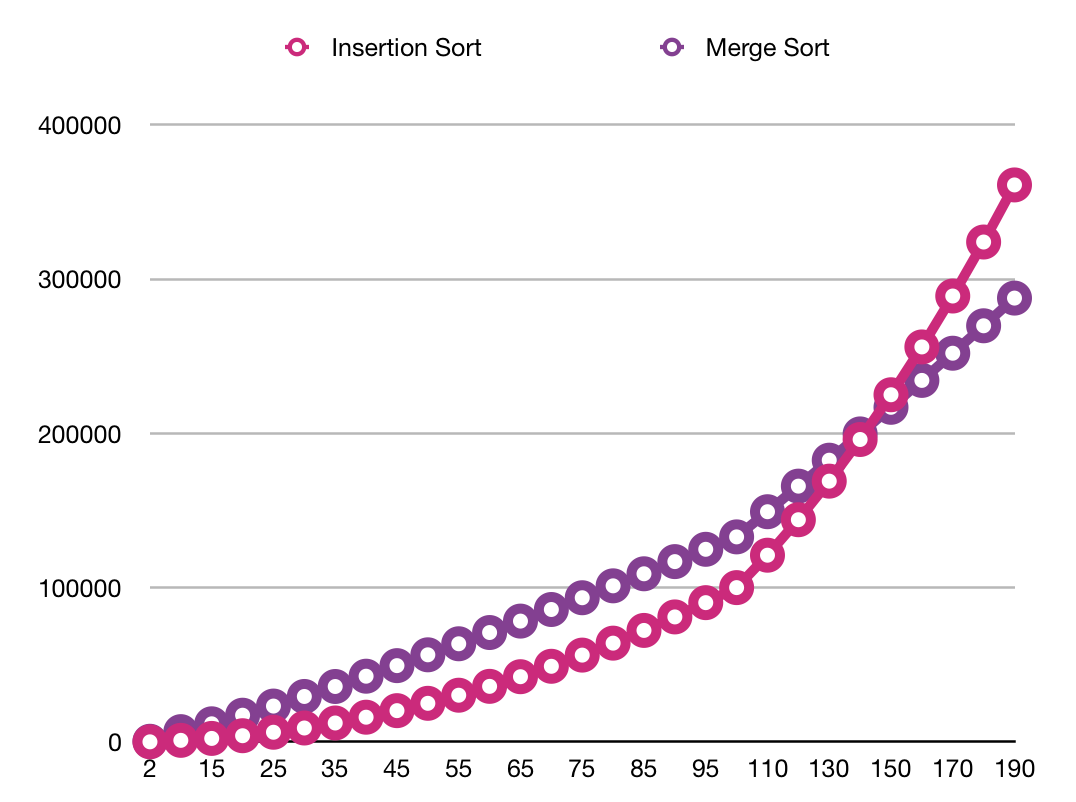
\includegraphics[width=\textwidth]{efficiency}
    \caption{Asymptotic Comparison of running times of insertion sort and merge sort}
    
\end{figure}
\begin{table}
\begin{center}
\begin{tabular}{|c|c|c|c|}
\hline 
\textit{N} & Insertion Sort & Merge Sort & Efficient Algorithm \\ 
\hline 
2 & 40 & 400 & Insertion \\
10 & 1000 & 6643.85619 & Insertion \\
15 & 2250 & 11720.6718 & Insertion \\
20 & 4000 & 17287.7124 & Insertion \\
25 & 6250 & 23219.2809 & Insertion \\
30 & 9000 & 29441.3436 & Insertion \\
35 & 12250 & 35904.9811 & Insertion \\
40 & 16000 & 42575.4248 & Insertion \\
45 & 20250 & 49426.6779 & Insertion \\
50 & 25000 & 56438.5619 & Insertion \\
55 & 30250 & 63594.9568 & Insertion \\
60 & 36000 & 70882.6871 & Insertion \\
65 & 42250 & 78290.7816 & Insertion \\
70 & 49000 & 85809.9622 & Insertion \\
75 & 56250 & 93432.2804 & Insertion \\
80 & 64000 & 101150.85 & Insertion \\
85 & 72250 & 108959.646 & Insertion \\
90 & 81000 & 116853.356 & Insertion \\
95 & 90250 & 124827.257 & Insertion \\
100 & 100000 & 132877.124 & Insertion \\
110 & 121000 & 149189.914 & Insertion \\
120 & 144000 & 165765.374 & Insertion \\
130 & 169000 & 182581.563 & Insertion \\
140 & 196000 & 199619.924 & Insertion \\
150 & 225000 & 216864.561 & Merge \\
160 & 256000 & 234301.699 & Merge \\
170 & 289000 & 251919.292 & Merge \\
180 & 324000 & 269706.711 & Merge \\
190 & 361000 & 287654.513 & Merge \\
 \hline
\end{tabular}
\caption{Running time for insertion sort and merge sort with $c_{1}\ =\ 10\ and\ c_{2}\ =\ 200$}
\label{table:1}
\end{center}
\end{table}
\subsection{Another Reason to Analyze Algorithms}
Even if speed and cost were not an issue we still have to study algorithms to show they actually terminate and do so with the right answer (i.e., proof their correctness). In reality, though, both speed and cost associated with algorithms is an issue and we want to study it.
\subsection{Example: Analysis of Insertion Sort}
To recap, analyzing algorithm refers to figuring out the amount of resource required to execute it. Analysis of algorithm in relation to its time complexity, hence, refers to the time it takes to execute the algorithm. Further since we assume all elementary operations (i.e., those operations defined by the computational model) as to take a a single unit of time, counting the number of these operations performed by the algorithm will give as the total time required to execute the algorithm. 
\lstinputlisting[language=C]{code/insertionSort.pseudo}
\par To illustrate this process in action, in this section, we will analyze the time complexity of insertion sort with an implementation presented above. The time taken by the insertion sort procedure depends on
\begin{itemize}
\item \textbf{Input size}: sorting a thousand numbers takes longer than ten
\item \textbf{Input sort status}: sorting an input already nearly sorted would be faster than a reversely sorted input.
\end{itemize}
\par In general the running time of a program depends on the \textbf{\textit{input size}}. Hence we need to describe running time as a function of input size.The notion of input size depends on the problem being studied. For many problems it is the number of items in the input. For others such as multiplying integers the best measure is the total number of bits and in other cases such as graph problems the input will described by more than one number (i.e., number of vertices and edges). We shall indicate which input size measure is being used with each problem we study.
\par  The running time of an algorithm on a particular input is the number of primitive operations or steps executed. It is convenient to define the notion of steps to make it machine-independent. It take a constant time to execute each line of our pseudocode but one line may take a different amount of time that the other. Let say line $i$ of the pseudocode takes $c{i}$ to execute and the inner while loop tests $t_{j}$ times for the $ j^{th}$ item. 
\begin{figure}[h]
    \centering
    \label{fig:InsertionRunTime}
    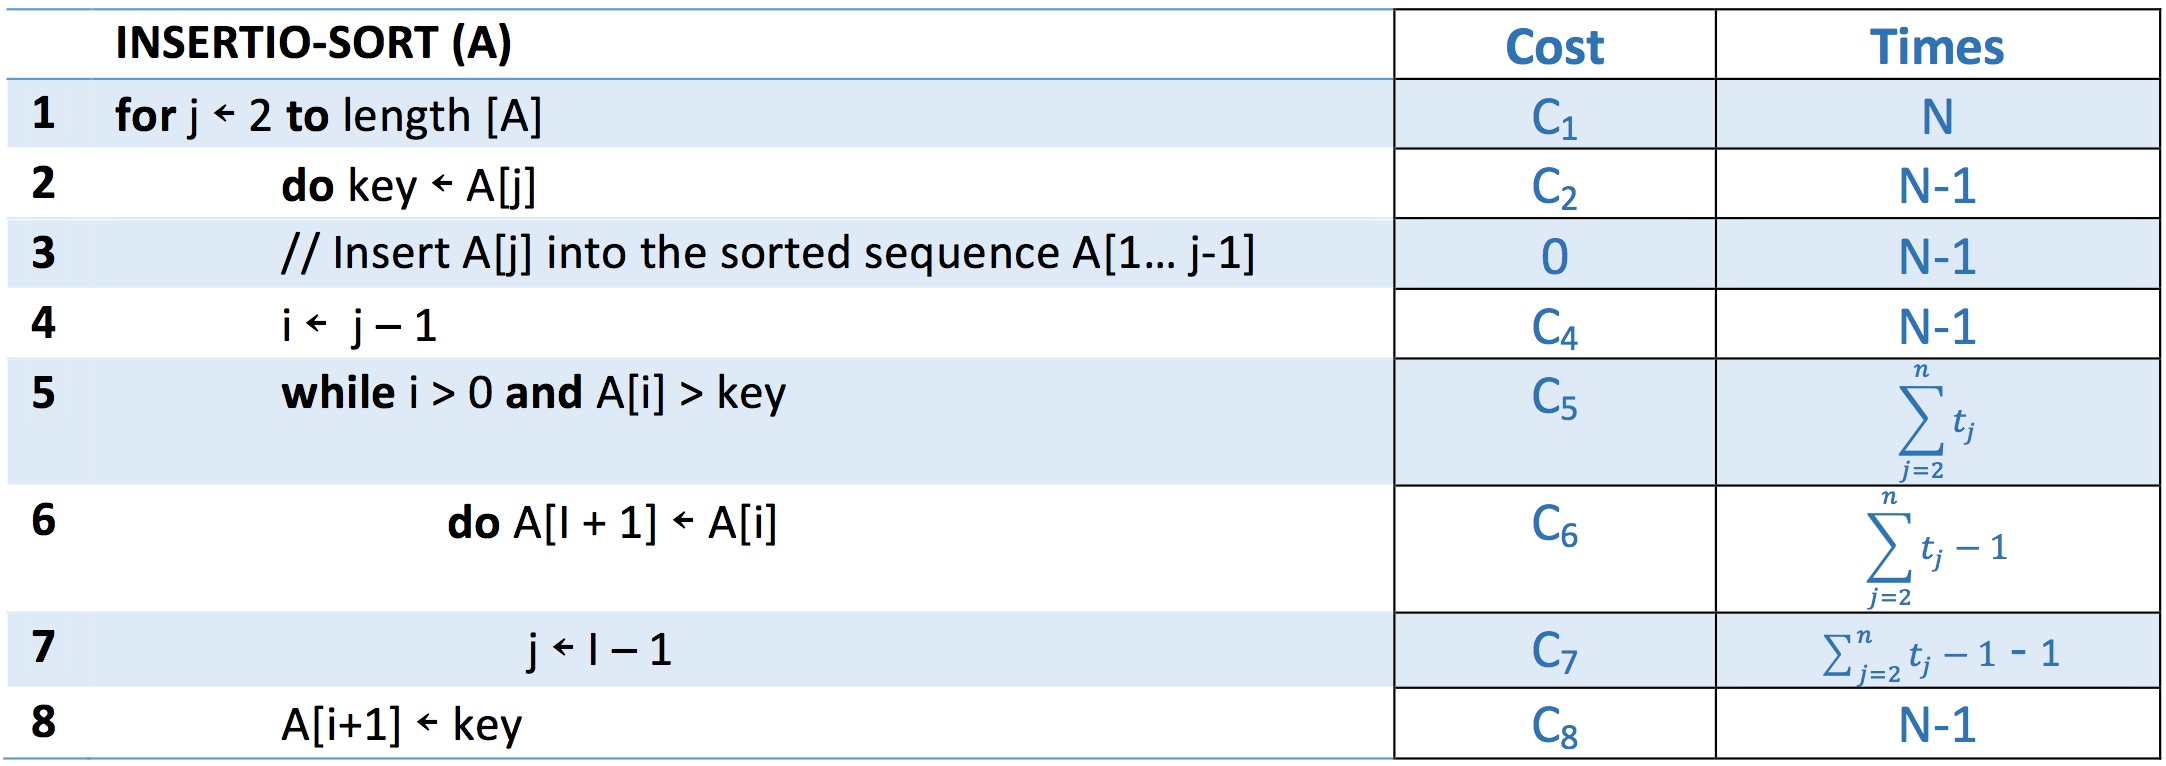
\includegraphics[width=\textwidth]{InsertionRunTime}
    \caption{Running Time Analysis of Insertion Sort}   
\end{figure}
\par Based on {Figure \ref{fig:InsertionRunTime}} the total running time of the algorithm is the sum of running times of each statement executed
\begin{equation}
\begin{aligned}
T(n) = C_{1}n\  +\  C_{2}(n-1) + C_{4}(n-1)\ +\ C_{5}\sum_{j=2}^{n} t_{j}\  +\\
 C_{6}\sum_{j=2}^{n} (t_{j} -1)\ +\ C_{7}\sum_{j=2}^{n} (t_{j}\ -\ 1)\ +\ C_{8}(n - 1)
\end{aligned}
\end{equation}
\par As stated in previously the running time of a program depends on the input size and in this case the level of sorting it already is in. For insertion sort the best case is when the input is already sorted in which case for each $j = 2,3 ... n\ A[i]\ <\ key$ in the first iteration of the while loop $(i = j - 1)$ hence $t_{j} = 1$ leading to the following equation.
\begin{equation}
T(n) = C_{1}n\  +\  C_{2}(n-1) + C_{4}(n-1)\ +\ C_{5}(n-1)\  +\ C_{8}(n - 1)
\end{equation}
\begin{equation}
T(n) = (C_{1}\  +\  C_{2}\ +\ C_{4}\  +\ C_{5}\  +\ C_{8}\ )n - (C_{2}\ +\ C_{4}\  +\ C_{5}\  +\ C_{8}\ )
\end{equation}
\par If the array was in reverse order the algorithm will face its worst case results since we must compare each $A[j]$ with all the elements in the sorted portion of the array
\begin{equation}
\sum_{j=2}^{n}\ j\ = \frac{n(n\ +\ 1)}{2}\ -\ 1
\end{equation}
\begin{equation}
\sum_{j=2}^{n}\ j\ -\ 1\ = \frac{n(n\ -\ 1)}{2}
\end{equation}
\begin{equation}
\begin{aligned}
T(n) = C_{1}n\  +\  C_{2}(n\ -\ 1)\ +\ C_{4}(n\ -\ 1)\  +\ C_{5}(\frac{n(n-1)}{2}\ -\ 1)\ +\\
C_{6}(\frac{n(n-1)}{2})\ +\ C_{7}(\frac{n(n-1)}{2})\ +\ C_{8}(n\ -\ 1)
\end{aligned}
\end{equation}
\begin{equation}
\begin{aligned}
T(n) = (\frac{C_{5}}{2}\  +\  \frac{C_{6}}{2}\ +\ \frac{C_{7}}{2})n^2\ +\ (C_{1}\ +\ C_{2}\
 +\ C_{4}\ +\ \frac{C_{5}}{2}\ -\\
  \frac{C_{6}}{2}\ +\ \frac{C_{7}}{2}\ +\ C_{8})n\ -\ (C_{2}\ +\ C_{4}\ +\ C_{5}\ +\ C_{8}\ ) 
\end{aligned}
\end{equation}
\par So we can express the worst case running time as $an^2\ +\ bn\ +\ c$ if we replace the coefficients in the above equation with constants $a$, $b$ and $c$. We used some simplifying abstractions to ease our analysis by ignoring actual statement cost and even the abstracts costs $C_{i}$. We normally even further simplify this by only considering \textbf{\textit{rate of growth}} or \textbf{\textit{order of growth}} instead of the actual running time. We shall do this because what we really want to know is whom our algorithm performance compared to others for large input sizes.
\par We therefore only consider the leading term $an^2$ since the lower order terms (i.e., $bn$ and $c$) will have relatively insignificant for the large values of n compared to the first once. We even ignore the coefficient a due to similar reasons as to why we ignored the other terms to be left with $n^2$ which we consider as our order of growth. We call this the theta notation and it is presented as $\Theta(n^2)$
\section{Correctness of An Algorithm}
\subsection{Introduction}
After designing algorithms in addition to analyzing the resource requirement one should proof its correctness. Proving the correctness means that showing that the algorithm halts and halts with correct answer for all valid inputs. In this course the primary technique we will use for proving correctness of an algorithm is \textbf{\textit{mathematical induction}}.
\par Mathematical Induction is a mathematical proof technique used to prove a given statement about any well-ordered set. Most commonly, it is used to establish statements for the set of all natural numbers. Mathematical induction is a form of direct proof, usually done in two steps. When trying to prove a given statement for a set of natural numbers, the first step, known as the \textbf{base case}, is to prove the given statement for the first natural number. The second step, known as the \textit{inductive step}, is to prove that, if the statement is assumed to be true for any one natural number, then it must be true for the next natural number as well. Having proved these two steps, the rule of inference establishes the statement to be true for all natural numbers. In common terminology, using the stated approach is refers to as using the \textit{Principle of Mathematical Induction}.
\par in addition to these two steps in the conventional mathematical induction, while proving correctness of algorithm we add a third step to check the termination of the algorithm. 
\subsection{Loop Invariant}
A loop invariant is a property of a program loop that is true before (and after) each iteration. It is a logical assertion, sometimes checked within the ode by an assertion call. Knowing its invariant(s) is essential in understanding the effect of a loop. What is more, it is what we will use to prove in the base case and the inductive step. 
\par In the pseudocode of insertion sort presented earlier, $j$ indicates the current card being inserted. At the beginning of the outer loop (i.e., for loop), which is indexed by $j$, the sub array containing elements $A[1... j-1]$ consists of the currently sorted hand and elements $A[j+1 ...n]$ correspond to the pile of cards still on the table. In fact elements $A[1... j-1]$ are the elements originally positions 1 through $j-1$ but now in a sorted order.
\par We state these properties formally as \textit{\textbf{loop invariants}}
\begin{quotation}
At the start of each iteration of the for loop of lines 2-8, the subarray $A[1... j-1]$ consists of the elements originally in $A[1 .. j-1]$ \textbf{\textit{but in a sorted order}}
\end{quotation}
We use these loop invariants to help us understand why an algorithm is \textbf{\textit{correct}}.
\subsection{Correctness Proof}
We must show three things about a loop invariant to proof an algorithm’s correctness
\begin{itemize}
\item \textbf{Initialization}: It is true prior to the first iteration of the loop
\item \textbf{Maintenance}: If it is true before an iteration of the loop, it remains true before the next
iteration
\item \textbf{Termination}: when the loop terminates, the invariant gives us a useful property that
helps show that the algorithm is correct
\end{itemize}
\par Notice the similarity of this approach to mathematical induction in which you proof the \textit{\textbf{base case}} and then the \textbf{\textit{inductive step}}. Here showing the loop invariant holds for the first iteration is the base case and showing that the invariant holds from iteration to iteration is like the inductive case.
\par One important difference from mathematical induction is the third step in which we show the correctness for the termination case. In mathematical induction we show that the inductive step holds infinitely, here we stop the induction when the loop terminates.
\subsection{Example: Insertion Sort}
\lstinputlisting[language=C]{code/insertionSort.pseudo}
Using these properties we will show the correctness of insertion sort algorithm.
\begin{itemize}
\item \textbf{Loop Invariant}: At the $j^{th}$ iteration the elements $[1...j-1]$ are sorted relative to themselves.
\item \textbf{Initialization}: 
We start by showing that the loop invariant holds before the first loop iteration when $j\ =\ 2$. The subarray $[1 ... j-1]$, therefore, consists of just the single element $A[1]$, which in fact it the original element $A[1]$.  This array is sorted (trivial)
\item \textbf{Maintenance}:
In the algorithm the for loop works by moving $A[j-1],\ A[j-2],\ A[j-3]$ and so on by one position to the right until the right position for $A[j]$ is found at which point the value of $A[j]$ is inserted. More formally, though, it is required to show the loop invariant of the inner loop as well. Here, however, we will not go into such detail for the time being
\item \textbf{Termination}:
The outer loop end when $j$ exceeds $n$, i.e., when $j\ =\ n\ +\ 1$ substituting $n\ +\ 1$ for $j$ in the wording of loop invariant we have the $subarray A[1... n]$ consists of the elements originally in $A[1 .. n]$ but in a sorted order. But the subarray $A[1...n]$ is the entire array which means the entire array is sorted
\end{itemize}
\subsection{Example: Bubble Sort}
\lstinputlisting[language=C]{code/bubbleSort.pseudo}
Using mathematical induction we will show the correctness of bubble sort algorithm.
\begin{itemize}
\item \textbf{Loop Invariant}: At the $i^{th}$ iteration the last $i$ elements $[n-i,.....n]$ are sorted relative to themselves and are all greater than all elements in $[1, .....n-i-1]$.
\item \textbf{Initialization}: 
We start by showing that the loop invariant holds before the first loop iteration when $i\ =\ n-1$. The subarray $[n-i ... n]$, therefore, consists of no element as $n-n-1\ =\ n$, and $A[n]$ is empty  as we are using 0 based index.  This array is sorted (trivial)
\item \textbf{Maintenance}:
In the algorithm the inner for loop bubbles the maximum element from $A[0],\ A[1],\ A[2],\ ...\ A[i]$ to the end (i.e., the $i^{th}$ position. Which means if we assume the elements $i\ to\ n$ are sorted and they are all greater than all elements $0\ - i\ -\ 1$ in the $i^{th}$ iteration, then on the so on $(i\ +\ 1)^{th}$ iteration the biggest element from $A[0],\ A[1],\ A[2],\ ...\ A[i-1]$will be on $(i\ -\ 1)^{th}$ location making the lats $(i\ +\ 1)$ sorted hence maintaining the loop invariant.
\item \textbf{Termination}:
The outer loop end when $i$ becomes $0$ hence from the loop invariant we have when the loop terminates the last $n-0$ elements are sorted which means the entire list is sorted.
\end{itemize}
\subsection{Exercises}
\begin{enumerate}
\item Re-write the pseudocode of insertion sort procedure to sort into non- increasing instead of non-decreasing order
\item Analyze the running time of bubble sort algorithm presented in the previous chapter
\item Prove the correctness of selection sort algorithm presented in the previous chapter using mathematical induction.
\item Analyze the running time of selection sort algorithm presented in the previous chapter
\item Given the searching problem defined in previous class
\begin{enumerate}
\item Write the pesudocode for linear search, which scans through the sequence, looking for the item.
\item Using loop invariant, prove that your algorithms are correct
\item Write the pesudocode for binary search, which uses the divide and conquer technique.
\end{enumerate}
\item Consider the problem of adding two n-bit binary integers, stored in two n-element arrays A and $B$. The sum of the two integers should be stored in binary form in an $(\ n\ +\ 1)$ element array $C$. stat the problem formally and write pseudocode for adding the two integers
\end{enumerate}
\section{Growth Function}
\subsection{Asymptotic Notation}
In previous section we defined the running time of an algorithm on a particular input as the number of primitive operations or "steps" executed. Although we can sometimes determine the exact running time of an algorithm the extra precision is not usually worth the effort of computing it. For large enough inputs, the effects of the input size itself dominate the multiplicative constants and lower-order terms of an exact running time.
\par The order of growth of the running time of an algorithm gives a simple characterization of the algorithm's efficiency and also allows us to compare the relative performance of alternative algorithms. Once the input size n becomes large enough, merge sort, with its $\Theta (n\log n)$ worst-case running time beats insertion sort, whose worst-case running time is $\Theta (n^{2})$. When we look at input sizes large enough to make only the order of growth of the running time relevant, we are studying the \textbf{\textit{asymptotic efficiency}} of algorithms. That is, we are concerned with how the running time of an algorithm increases with the size of the input as it increases without bound. Usually, an algorithm that is asymptotically more efficient will be the best choice for all but very small inputs. Hence, we will use asymptotic notation primarily to describe the running times of algorithms.
\par In this section we will discuss several standard methods for simplifying the asymptotic analysis of algorithms. We start by defining several types of "\textbf{\textit{asymptotic notations}}" of which we have already seen an example in, $\Theta$ – notation (i.e., Theta – notation). We then present several notational conventions used throughout this course, and then we review the behavior of functions that commonly arise in the analysis of algorithms.
\par \textbf{\textit{Bachmann-Landau Notation}} or \textbf{\textit{Asymptotic Notation}} is a family of notations invented by \textit{Paul Bachmann, Edmund Landau}, and others, that describes the limiting behavior of a function when the argument tends towards a particular value or infinity.
\par In this course, the functions to which we apply asymptotic notation will usually characterize the running times of algorithms. But asymptotic notation can apply to functions that characterize some other aspect of algorithms (the amount of space they use, for example), or even to functions that have nothing whatsoever to do with algorithms.
\par Moreover, the notations we use to describe the asymptotic running time of an algorithm are defined in terms of functions whose domains are the set of natural numbers $N = {0, 1, 2...}$.
\par Even when we use asymptotic notation to apply to the running time of an algorithm, we need to understand which running time we mean. Sometimes we are interested in the worst-case running time. Often, however, we wish to characterize the running time no matter what the input. In other words, we often wish to make a blanket statement that covers all inputs, not just the worst case. We shall see asymptotic notations that are well suited to characterizing running times no matter what the input.
\subsubsection{$O$ – notation (i.e., Big-oh notation )}
The $O$ - notation asymptotically bounds a function from above. To put it more formally, for a given function $g(n)$, we denote by $\O(g(n))$ (pronounced "big-oh of $g$ of $n$" or sometimes just "oh of $g$ of $n$") the set of functions
\begin{equation}
\begin{aligned}
O(g(n)) = f(n)\ :\ there\ exists\ posetive\ constant\ \mathit{c}\ and\ n_{o}\\
 such\ that\ 0\ \leq\ f(n)\ cg(n)\ for\ all\ n\ \geq\ n_{o}
\end{aligned}
\end{equation}
We use $\Omega$-notation to give an upper bound on a function, to within a constant factor. This means for sufficiently large n values (i.e., $n \geq n_{o}$) there is a constant value $c$ such that the function $f(n)$ is below $cg(n)$. {\color{red} Figure 1 (a)} shows the intuition behind $\O$-notation. For all values $n$ at and to the right of $n_{o}$, the value of the function $f(n)$ is on or below $cg(n)$.
\par We write $f(n) = \O (g(n))$ to indicate that a function $f(n)$ is a member of the set $O(g(n))$. However, since we said $O(g(n))$ is a set of functions, we could write $f(n) \epsilon \O(g(n))$ to indicate that $f(n)$ is a member of $O(g(n))$. However, throughout this course and most literatures in algorithm analysis "$f(n) = O(g(n))$" is used to express the same notion.
\subsubsection{$\Omega$-notation (i.e., Big-omega notation )}
{\color{red} Content Under Development}
\subsubsection{$\Theta$-notation (i.e., Theta notation )}
{\color{red} Content Under Development}
\subsubsection{$o$-notation (i.e., Little-oh notation )}
{\color{red} Content Under Development}
\subsubsection{$\omega$-notation (i.e., Little-omega notation )}
{\color{red} Content Under Development}
\subsubsection{Asymptotic Notation in Equations and Inequalities}
{\color{red} Content Under Development}
\subsubsection{Comparing functions}
{\color{red} Content Under Development}
\subsection{Standard Notions and Common Functions}
{\color{red} Content Under Development}
\subsubsection{Monotonicity}
{\color{red} Content Under Development}
\subsubsection{Floors and Ceilings}
{\color{red} Content Under Development}
\subsubsection{Modular Arithmetic}
{\color{red} Content Under Development}
\subsubsection{Polynomials}
{\color{red} Content Under Development}
\subsubsection{Exponentials}
{\color{red} Content Under Development}
\subsubsection{Factorials}
{\color{red} Content Under Development}
\subsubsection{Functional Iteration}
{\color{red} Content Under Development}
\subsubsection{The Iterated Logarithm Function}
{\color{red} Content Under Development}
\subsubsection{Fibonacci Numbers}
We define the \textbf{\textit{Fibonacci Numbers}} by the following recurrence:
\section{Summary}
In this we discussed what we men by analyzing algorithms and why we do so. We discussed how we prove the correctness of algorithm using a variation mathematical induction. In this regard we highlighted what loop invariant refers to and how we use it in the base case and induction step of our proof. We also covered the concept of asymptotic notations and some of the common mathematical functions deemed necessary for the course.
\subsection{Review Questions}
{\color{red} Content Under Development}
\subsection{Further Reading}
{\color{red} Content Under Development}
\part{Graphs}
%%Graph problems pervade computer science, and algorithms for working with them are fundamental to the field. Hundreds of interesting computational problems are couched in terms of graphs. In this part, we touch on a few of the more significant ones. In the first chapter we will see how we can represent a graph in a computer and we discuss algorithms based on searching a graph using either breadth-first search or depth-first search. The chapter, also, covers sample applications of these traversal algorithms. Implementations of these algorithms and concepts is also presented in this chapter 
%Add more chapters%
\chapter{Representations and Traversal}
\section{Introduction}
This chapter presents methods for representing a graph and for searching a graph. Searching a graph means systematically following the edges of the graph so as to visit the vertices of the graph. A graph-searching algorithm can discover much about the structure of a graph. Many algorithms begin by searching their input graph to obtain this structural information. Several other graph algorithms elaborate on basic graph searching. Techniques for searching a graph lie at the heart of the field of graph algorithms.\par
The first section discusses the two most common computational representations of graphs: as adjacency lists and as adjacency matrices. The second section, then, presents a simple graph-searching algorithm called breadth-first search and shows how to create a breadth-first tree. The third section presents depth-first search and proves some standard results about the order in which depth-first search visits vertices. The forth section The fifth section provides some sample real application of these traversal algorithms, For depth-first search we see topologically sorting a directed acyclic graph. A second application of depth-first search, finding the strongly connected components of a directed graph. We also see how we can test bipartiteness of graphs using Breadth-first search.\par
When we characterize the running time of a graph algorithm on a given graph $G = (V, E)$, we usually measure the size of the input in terms of the number of vertices $|V|$ and the number of edges $|E|$ of the graph. That is, we describe the size of the input with two parameters, not just one. We adopt a common notational convention for these parameters. Inside asymptotic notation (such as $O-notation$ or ‚$\theta-notation$), and only inside such notation, the symbol V denotes $|V|$ and the symbol E denotes $|E|$. For example, we might say, "the algorithm runs in time $O(VE)$" meaning that the algorithm runs in time $O(|V| |E|)$. This convention makes the running-time formulas easier to read, without risk of ambiguity.\par
Another convention we adopt appears in pseudocode. We denote the vertex set of a graph $G$ by $G.V$ and its edge set by $G.E$. That is, the pseudocode views vertex and edge sets as attributes of a graph.
\section{Basic Definitions and Representation }
Our focus in this course is on problems with a discrete flavor. Just as continuous mathematics is concerned with certain basic structures such as real numbers , vectors, and matrices, discrete mathematics has developed basic combinatorial structures that lie at the heart of the subject. One of the most fundamental  and expressive of these is the \textit{graph}.\par
The more one works with graphs, the more one tends to see them everywhere. Thus, we begin by introducing the basic definitions surrounding graphs, and list a spectrum of different algorithmic settings where graphs arise naturally. We then discuss some basic algorithmic primitives for graphs, beginning with the problem of connectivity and developing some fundamental graph search techniques.\par
A graph $G$ is simply a way of encoding pairwise relationships among a set of objects: it consists of a collection $V$ of nodes and a collection $E$ of edges, each of which "joins" two of the nodes. We thus represent an edge $e \in E$ as a two-element subset of $V: e = {u, v}$ for some $u,v \in V$, where we call $u$ and $v$ the ends of $e$.\par
Edges in a graph indicate a symmetric relationship between their ends. Often we want to encode asymmetric relationships, and for this we use the closely related notion of a \textit{directed graph}. A directed graph $G'$ consists of a set of nodes $V$ and a set of directed edges $E'$. Each $e' \in E'$ is an ordered pair $(u, v)$; in other words, the roles of $u$ and $v$ are not interchangeable, and we call $u$ the tail of the edge and $v$ the head. We will also say that edge $e'$ leaves node $u$ and enters node $v$.\par
When we want to emphasize that the graph we are considering is not directed, we will call it an \textit{undirected graph}; by default, however, the term "graph" will mean an undirected graph. It is also worth mentioning two warnings in our use of graph terminology. First, although an edge $e$ in an undirected graph should properly be written as a set of nodes ${u, v}$, one will more often see it written in the notation used for ordered pairs: $e = (u, v)$. Second, a node in a graph is also frequently called a vertex; in this context, the two words have exactly the same meaning.\par 
\textbf{\textit{Examples of Graphs}} Graphs are very simple to define: we just take a collection of things and join some of them by edges. But at this level of abstraction, it's hard to appreciate the typical kinds of situations in which they arise. Thus, we propose the following list of specific contexts in which graphs serve as important models. The list covers a lot of ground, and it's not important to remember everything on it; rather, it will provide us with a lot of useful examples against which to check the basic definitions and algorithmic problems that we'll be encountering later in the chapter. Also, in going through the list, it's useful to digest the meaning of the nodes and the meaning of the edges in the context of the application. In some cases the nodes and edges both correspond to physical objects in the real world, in others the nodes are real objects while the edges are virtual, and in still others both nodes and edges are pure abstractions.
\begin{enumerate}
\item \textit{Transportation networks}. The map of routes served by an airline carrier naturally forms a graph: the nodes are airports, and there is an edge from $u to v$ if there is a nonstop flight that departs from $u$ and arrives at $v$. Described this way, the graph is directed; but in practice when there is an $edge (u, v)$, there is almost always an $edge (v, u)$, so we would not lose much by treating the airline route map as an $undirected$ graph with edges joining pairs of airports that have nonstop flights each way. Looking at such a graph (you can generally find them depicted in the backs of in-flight airline magazines), we'd quickly notice a few things: there are often a small number of hubs with a very large number of incident edges; and it's possible to get between any two nodes in the graph via a very small number of intermediate stops.\par
Other transportation networks can be modeled in a similar way. For example, we could take a rail network and have a node for each terminal, and an edge joining $u and v$ if there's a section of railway track that goes between them without stopping at any intermediate terminal. The standard depiction of the subway map in a major city is a drawing of such a graph.
\item \textit{Communication networks}  A collection of computers connected via a communication network can be naturally modeled as a graph in a few different ways. First, we could have a node for each computer and an edge joining $u and v$ if there is a direct physical link connecting them. Alternatively, for studying the large-scale structure of the Internet, people often define a node to be the set of all machines controlled by a single Internet service provider, with an edge joining $u and v$ if there is a direct peering relationship between them roughly, an agreement to exchange data under the standard \textbf{\textit{BGP}} protocol that governs global Internet routing. Note that this latter network is more "virtual" than the former, since the links indicate a formal agreement in addition to a physical connection.\par
In studying wireless networks, one typically defines a graph where the nodes are computing devices situated at locations in physical space, and there is an edge from $u to v$ if $v$ is close enough to $u$ to receive a signal from it. Note that it's often useful to view such a graph as directed, since it may be the case that $v$ can hear $u's$ signal but $u$ cannot hear $v's$ signal (if, for example, $u$ has a stronger transmitter). These graphs are also interesting from a geometric perspective, since they roughly correspond to putting down points in the plane and then joining pairs that are close together.
\item \textit{Information networks}.The World Wide Web can be naturally viewed as a directed graph, in which nodes correspond to Web pages and there is an edge from $u to v$ if u has a hyperlink to $v$. The directedness of the graph is crucial here; many pages, for example, link to popular news sites, but these sites clearly do not reciprocate all these links. The structure of all these hyperlinks can be used by algorithms to try inferring the most important pages on the Web, a technique employed by most current search engines.\par
The hypertextual structure of the Web is anticipated by a number of information networks that predate the Internet by many decades. These include the network of cross-references among articles in an encyclopedia or other reference work, and the network of bibliographic citations among scientific papers.
\item \textit{Social networks} Given any collection of people who interact (the employees of a company, the students in a high school, or the residents of a small town), we can define a network whose nodes are people, with an edge joining $u and v$ if they are friends with one another. We could have the edges mean a number of different things instead of friendship: the undirected $edge(u, v) $ could mean that $u and v$ have had a romantic relationship or a financial relationship; the directed $edge(u, v)$ could mean that $u$ seeks advice from $v$, or that $u$ lists $v$ in his or her e-mail address book. One can also imagine bipartite social networks based on a notion of affiliation: given a set $X$ of people and a set $Y$ of organizations, we could define an edge between $u \in X$ and $v \in Y$ if person u belongs to organization $v$.
\par Networks such as this are used extensively by sociologists to study the dynamics of interaction among people. They can be used to identify the most "influential" people in a company or organization, to model trust relationships in a financial or political setting, and to track the spread of fads, rumors, jokes, diseases, and e-mail viruses.
\item \textit{Dependency networks} It is natural to define directed graphs that capture the inter-dependencies among a collection of objects. For example, given the list of courses offered by a college or university, we could have a node for each course and an edge from $u to v$ if $u$ is a prerequisite for $v$. Given a list of functions or modules in a large software system, we could have a node for each function and an edge from $u to v$ if $u$ invokes $v$ by a function call. Or given a set of species in an ecosystem, we could define a graph a food web in which the nodes are the different species and there is an edge from $u to v$ if $u$ consumes $v$.
\end{enumerate}
This is far from a complete list, too far to even begin tabulating its omissions. It is meant simply to suggest some examples that are useful to keep in mind when we start thinking about graphs in an algorithmic context.\par
\textbf{\textit{Paths and Connectivity}} One of the fundamental operations in a graph is that of traversing a sequence of nodes connected by edges. In the examples just listed, such a traversal could correspond to a user browsing Web pages by following hyperlinks; a rumor passing by word of mouth from you to someone halfway around the world; or an airline passenger traveling from Addis Ababa to Houston on a sequence of flights.\par
\begin{figure}[h]
    \centering
    \label{fig:simpleGraph1}
    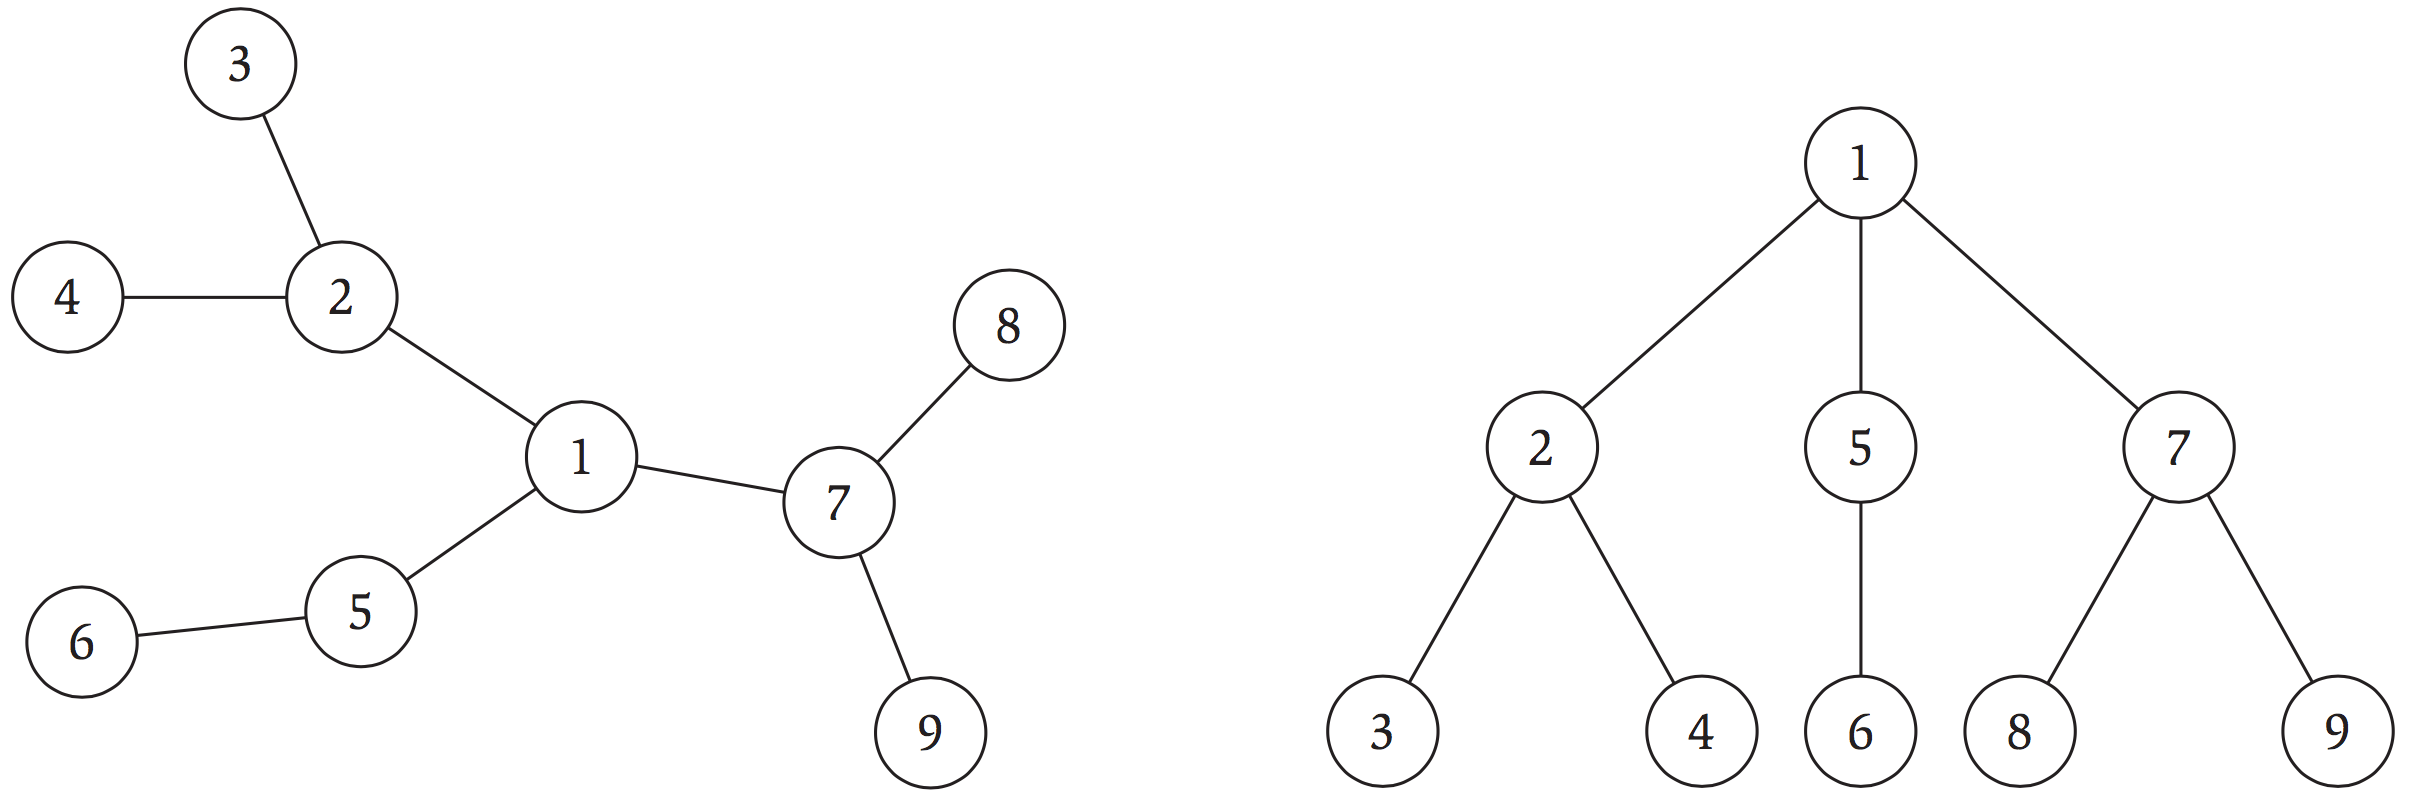
\includegraphics[width=\textwidth]{simpleGraph1}
    \caption{Two drawings of the same tree. On the right, the tree is rooted at node 1.}
\end{figure}
With this notion in mind, we define a path in an undirected graph $G=(V,E)$ to be a sequence $P$ of 
nodes $v_{1},v_{2}, ..., v_{k-1}, v_{k}$ with the property that each consecutive pair $v_{i} , v_{i+1} $ is  joined by an edge in $G$. $P$ is often called a path from $v_{1} to v_{k}$, or a $v_{1}-v_{k}$ path. For example, the nodes $4, 2, 1, 7, 8$ form a path in \ref{fig:simpleGraph1} . A path is called simple if all its vertices are distinct from one another. A cycle is a path $v_{1},v_{2},...,v_{k-1},v_{k}$ in which $k>2$,the first $k−1$ nodes are all distinct, and $v_{1} = v_{k}$ - in other words, the sequence of nodes "cycles back" to where it began. All of these definitions carry over naturally to directed graphs, with the following change: in a directed path or cycle, each pair of consecutive nodes has the property that $(v_{i} , v_{i+1})$ is an edge. In other words, the sequence of nodes in the path or cycle must respect the directionality of edges.\par 
We say that an \textbf{\textit{undirected}} graph is connected if, for every pair of nodes $u$ and $v$, there is a path from $u to v$. Choosing how to define connectivity of a directed graph is a bit more subtle, since it's possible for $u$ to have a path to $v$ while $v$ has no path to $u$. We say that a directed graph is strongly connected if, for every two nodes u and v, there is a path from u to v and a path from $v$ to $u$.\par
In addition to simply knowing about the existence of a path between some pair of nodes $u and v$, we may also want to know whether there is a short path. Thus we define the distance between two nodes $u and v$ to be the minimum number of edges in a $u-v$ path. (We can designate some symbol like $\infty$ to denote the distance between nodes that are not connected by a path.) The term distance here comes from imagining $G$ as representing a communication or transportation network; if we want to get from $u to v$, we may well want a route with as few "hops" as possible.\par
\textbf{\textit{Trees}} We say that an undirected graph is a tree if it is connected and does not contain a \textit{cycle}. For example, the two graphs pictured in \ref{fig:simpleGraphs} are trees. In a strong sense, trees are the simplest kind of connected graph: deleting any edge from a tree will disconnect it.\par 
For thinking about the structure of a tree $T$, it is useful to root it at a particular node $r$. Physically, this is the operation of grabbing $T$ at the node $r$ and letting the rest of it hang downward under the force of gravity, like a mobile. More precisely, we "orient" each edge of $T$ away from $r$; for each other node $v$, we declare the parent of $v$ to be the node $u$ that directly precedes $v$ on its path from $r$; we declare w to be a child of $v$ if $v$ is the parent of $w$. More generally, we say that $w$ is a descendant of $v$ (or $v$ is an ancestor of $w$) if $v$ lies on the path from the root to $w$;and we say that a node $x$ is a leaf if it has no descendants. Thus, for example, the two pictures in \ref{fig:simpleGraph1} correspond to the same tree T - the same pairs of nodes are joined by edges - but the drawing on the right represents the result of rooting $T$ at node 1.\par
Rooted trees are fundamental objects in computer science, because they encode the notion of a hierarchy. For example, we can imagine the rooted tree in \ref{fig:simpleGraph1}  as corresponding to the organizational structure of a tiny nine-person company; employees 3 and 4 report to employee 2; employees 2, 5, and 7 report to employee 1; and so on. Many Web sites are organized according to a tree-like structure, to facilitate navigation. A typical computer science department's Web site will have an entry page as the root; the People page is a child of this entry page (as is the Courses page); pages entitled Faculty and Students are children of the People page; individual professors' home pages are children of the Faculty page; and so on.\par
For our purposes here, rooting a tree T can make certain questions about $T$ conceptually easy to answer. For example, given a tree T on n nodes, how many edges does it have? Each node other than the root has a single edge leading "upward" to its parent; and conversely, each edge leads upward from precisely one non-root node. Thus we have very easily proved the following fact.
\begin{lemma}
Every n-node tree has exactly $n - 1$ edges.\par
\end{lemma}
In fact, the following stronger statement is true, although we do not prove it here.
\begin{lemma}
Let $G$ be an undirected graph on $n$ nodes. Any two of the following statements implies the third.
\end{lemma}
\begin{enumerate}
\item $G$ is connected.
\item $G$ does not contain a cycle.
\item $G$ has $n - 1$ edges.
\end{enumerate}
We now turn to the role of trees in the fundamental algorithmic idea of graph traversal.
\begin{figure}[h]
    \centering
    \label{fig:simpleGraph2}
    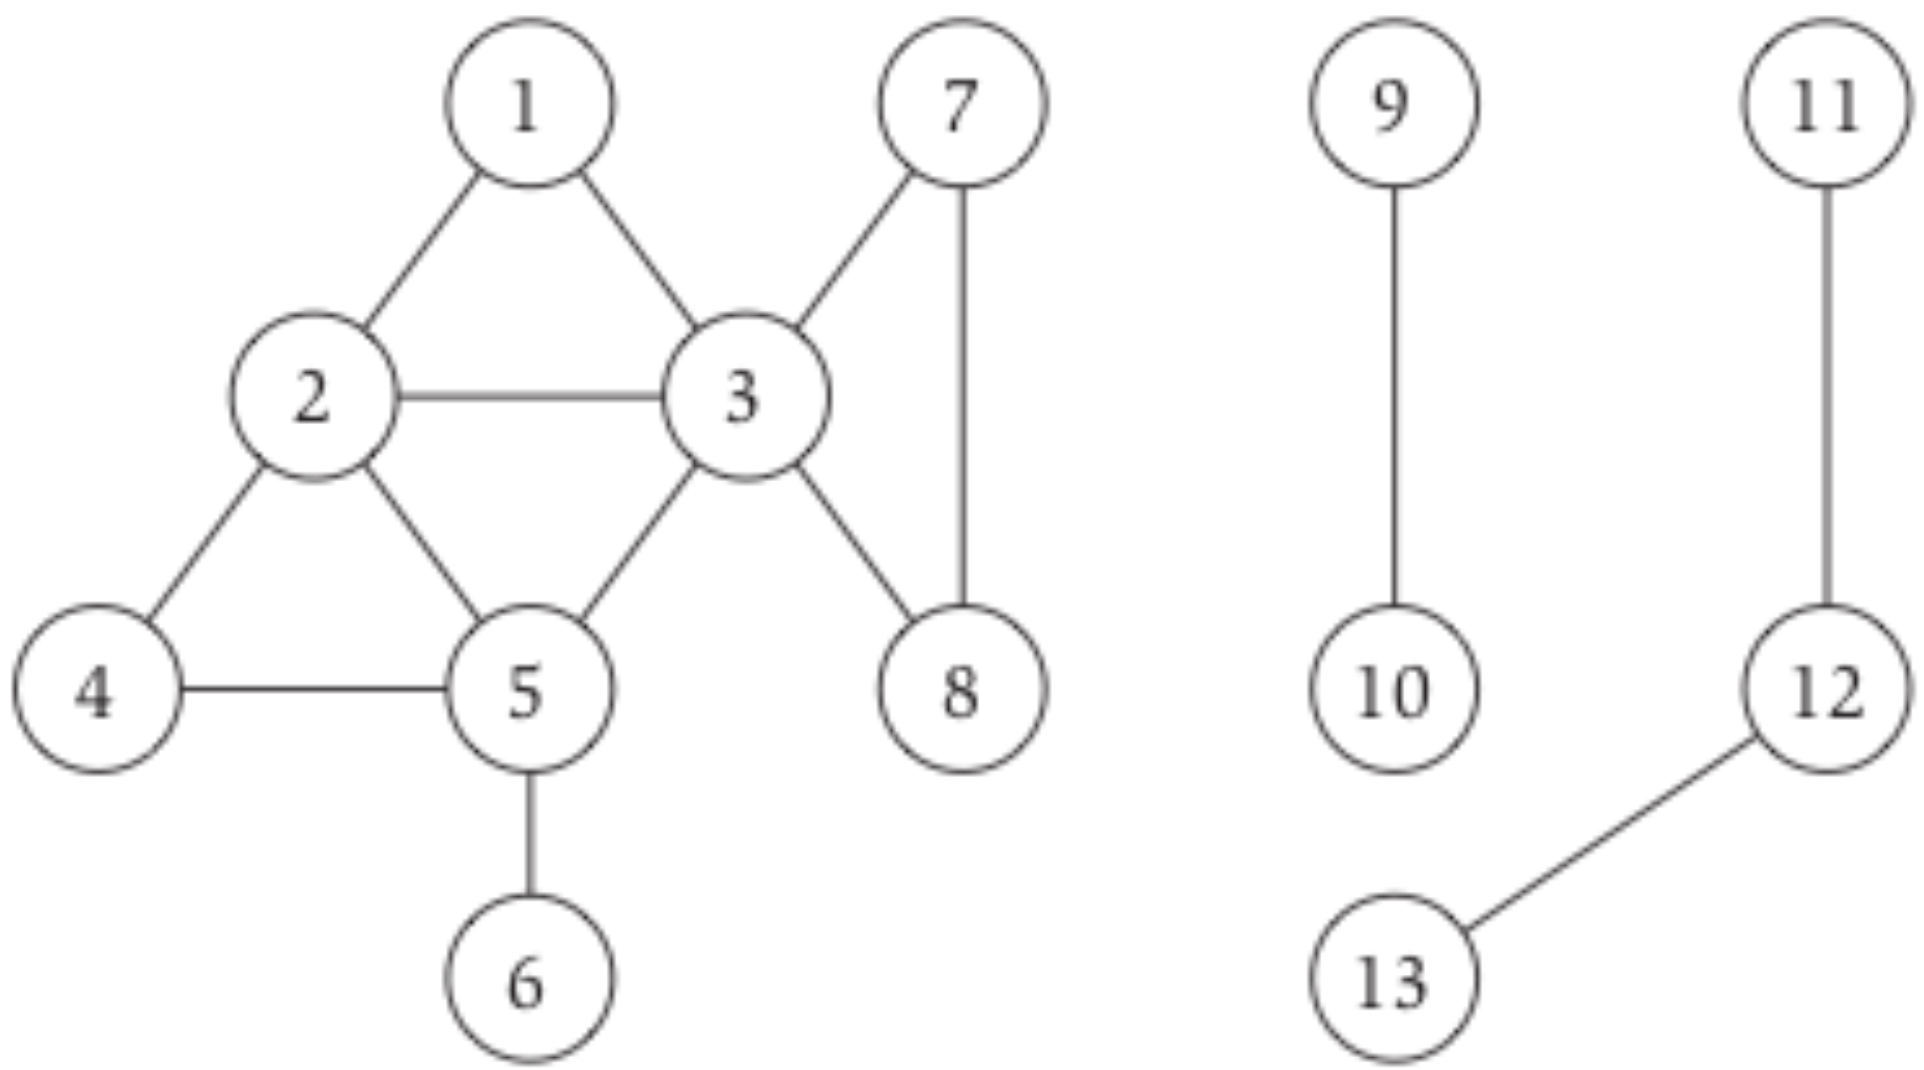
\includegraphics[width=\textwidth]{simpleGraph2}
    \caption{ In this graph, node 1 has paths to nodes 2 through 8, but not to nodes 9 through 13.}
\end{figure}
\subsection{Representations of Graphs}
We can choose between two standard ways to represent a graph $G = (V, E)$: as a collection of \textbf{\textit{adjacency lists}} or as an \textbf{\textit{adjacency matrix}}. Either way applies to both directed and undirected graphs. Because the adjacency-list representation provides a compact way to represent \textbf{\textit{sparse}} graphs - those for which $|E|$ is much less than $|V|^{2}$ - it is usually the method of choice. Most of the graph algorithms presented in this book assume that an input graph is represented in adjacency - list form. We may prefer an adjacency-matrix representation, however, when the graph is \textbf{\textit{dense}} - $|E|$ is close to $|V|^{2}$ - or when we need to be able to tell quickly if there is an edge connecting two given vertices. For example, two of the all-pairs shortest-paths algorithms presented later assume that their input graphs are represented by adjacency matrices.\par
\begin{figure}[h]
    \centering
    \label{fig:graphRepresentation1}
    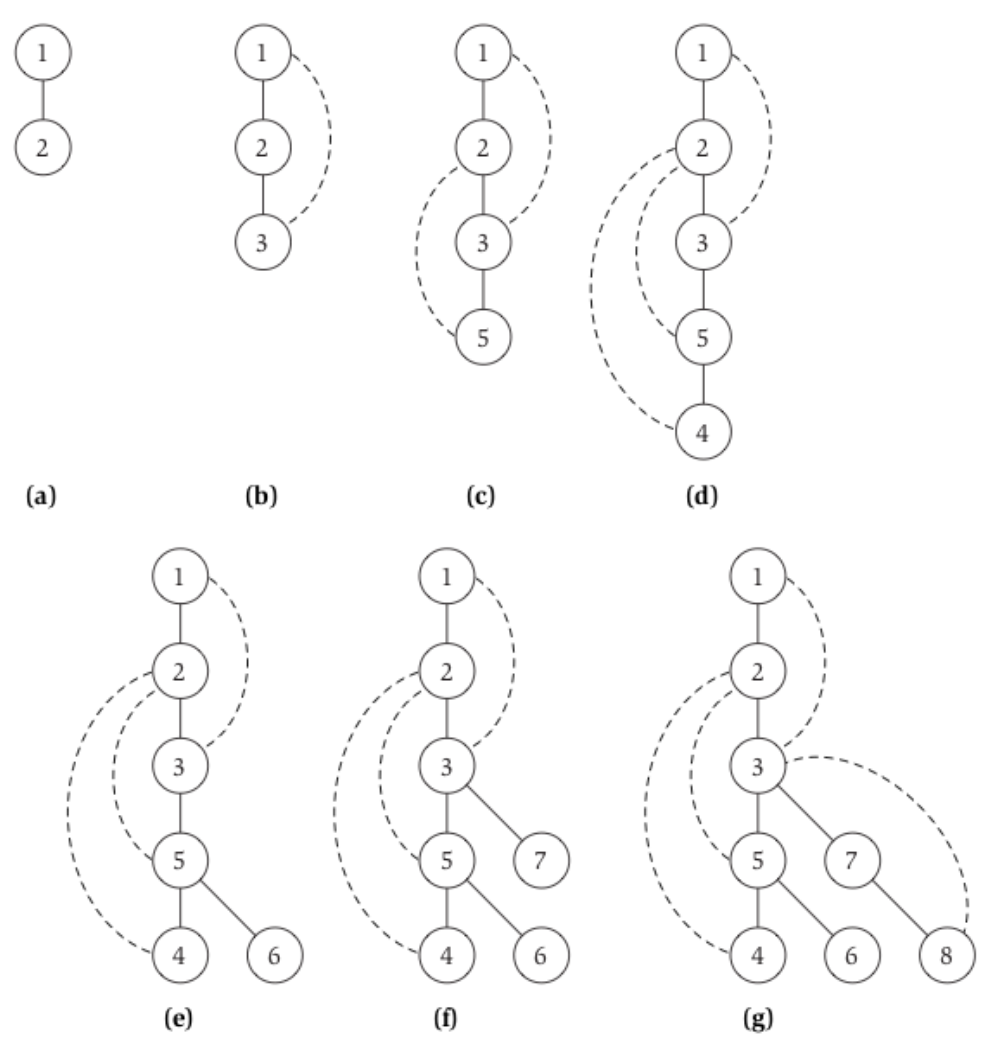
\includegraphics[width=\textwidth]{graphRepresentation1}
    \caption{ Two representations of an undirected graph. \textbf{(a)} An undirected graph G with 5 vertices and 7 edges. \textbf{(b)} An adjacency-list representation of G. \textbf{(c)} The adjacency-matrix representation of G.}
\end{figure}
\begin{figure}[h]
    \centering
    \label{fig:graphRepresentation2}
    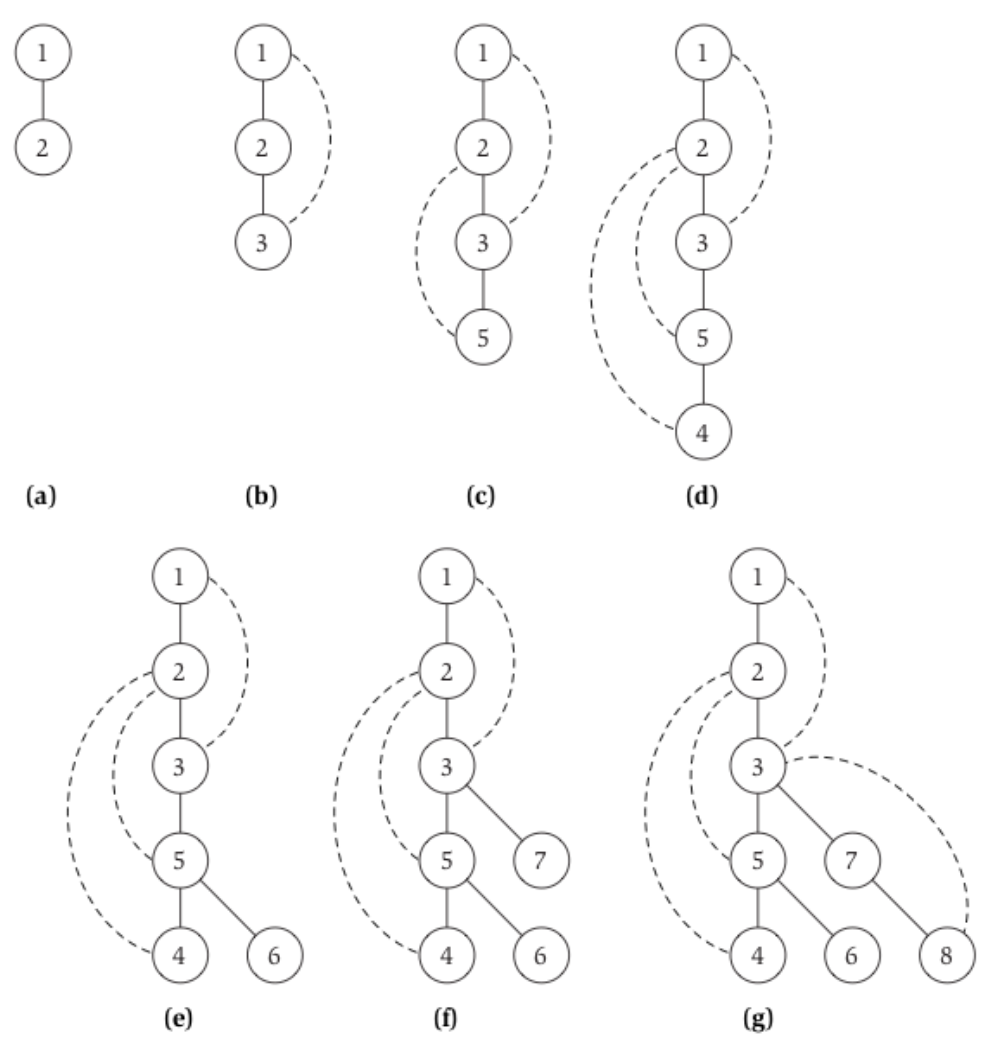
\includegraphics[width=\textwidth]{graphRepresentation2}
    \caption{ Two representations of a directed graph. \textbf{(a)} A directed graph G with 6 vertices and 8 edges. \textbf{(b)} An adjacency-list representation of G. \textbf{(c)} The adjacency-matrix representation of G.}
\end{figure}
The \textbf{\textit{adjacency-list representation}} of a graph $G = (V,E)$ consists of an array Adj of $V$ lists, one for each vertex in $V$. For each $u \in V$, the adjacency list $Adj[u]$ contains all the vertices $v$ such that there is an $edge (u,v) \in E$. That is, $Adj[u]$ consists of all the vertices adjacent to $u in G$. (Alternatively, it may contain pointers to these vertices.) Since the adjacency lists represent the edges of a graph, in pseudocode we treat the array $Adj$ as an attribute of the graph, just as we treat the edge set $E$. In pseudocode, therefore, we will see notation such as $G$. $Adj[u]$. Figure \ref{fig:graphRepresentation1} (b) is an adjacency-list representation of the undirected graph in Figure \ref{fig:graphRepresentation1}(a). Similarly, Figure \ref{fig:graphRepresentation2}(b) is an adjacency-list representation of the directed graph in Figure \ref{fig:graphRepresentation2}(a).\par
If $G$ is a directed graph, the sum of the lengths of all the adjacency lists is $|E|$, since an edge of the form $(u, v)$ is represented by having appear in $Adj[u]$. If $G$ is an undirected graph, the sum of the lengths of all the adjacency lists is $2|E|$, since if $(u,v)$ is an undirected edge, then $u$ appears in $u's$ adjacency list and vice versa. For both directed and undirected graphs, the adjacency-list representation has the desirable property that the amount of memory it requires is,$\theta(V+E)$.\par
We can readily adapt adjacency lists to represent \textbf{weighted graphs}, that is, graphs for which each edge has an associated \textbf{weight}, typically given by a \textbf{weight function} $w : E \rightarrow \rm I\!R $. For example, let $G=(V,E)$ be a weighted graph with weight function $w$. We simply store the weight $w(u, v)$ of the edge $(u, v) \in E $ E with vertex $v$ in $u's$ adjacency list. The adjacency-list representation is quite robust in that we can modify it to support many other graph variants.\par
A potential disadvantage of the adjacency-list representation is that it provides no quicker way to determine whether a given edge $(u,v)$ is present in the graph than to search for   in the adjacency list $Adj[u]$. An adjacency-matrix representation of the graph remedies this disadvantage, but at the cost of using asymptotically more memory. 
For the \textbf{\textit{adjacency-matrix representation}} of a graph $G=(V,E)$, we assume that the vertices are numbered $1,2,\dot \dot \dot, |V|$ in some arbitrary manner. Then the adjacency-matrix representation of a graph $G$ consists of a $|V| x |V|$ matrix $A =  (a_{ij})$ such that
\[
	a_{ij} = \begin{cases}
			1\qquad if (i,j) \in E, \\
			0\qquad otherwise
			\end{cases}
\]
Figures \ref{fig:graphRepresentation1}(c) and \ref{fig:graphRepresentation2}(c) are the adjacency matrices of the undirected and directed graphs in Figures \ref{fig:graphRepresentation1}(a) and \ref{fig:graphRepresentation2}(a), respectively. The adjacency matrix of a graph requires $\theta(V^{2})$ memory, independent of the number of edges in the graph.\par
Observe the symmetry along the main diagonal of the adjacency matrix in Figure \ref{fig:graphRepresentation1}(c). Since in an undirected graph, $(u,v)$ and $(v,u)$ represent the same edge, the adjacency matrix $A$ of an undirected graph is its own transpose: $A = A^{T}$. In some applications, it pays to store only the entries on and above the diagonal of the adjacency matrix, thereby cutting the memory needed to store the graph almost in half.\par
Like the adjacency-list representation of a graph, an adjacency matrix can represent a weighted graph. For example, if $G = (V, E)$ is a weighted graph with edge-weight function $w$, we can simply store the weight $(w, u)$ of the edge $(u,v) \in E$ as the entry in row $u$ and column of the adjacency matrix. If an edge does not exist, we can store a $NIL$ value as its corresponding matrix entry, though for many problems it is convenient to use a value such as $0\ or\ \infty$.\par
Although the adjacency-list representation is asymptotically at least as space-efficient as the adjacency-matrix representation, adjacency matrices are simpler, and so we may prefer them when graphs are reasonably small. Moreover, adjacency matrices carry a further advantage for unweighted graphs: they require only one bit per entry.
\subsubsection{Representing Attributes}
Most algorithms that operate on graphs need to maintain attributes for vertices and/or edges. We indicate these attributes using our usual notation, such as $v.d$ for an attribute $d$ of a vertex $v$. When we indicate edges as pairs of vertices, we use the same style of notation. For example, if edges have an attribute $f$ , then we denote this attribute for edge $(u,v)$ by $(u,v).f$. For the purpose of presenting and understanding algorithms, our attribute notation suffices.\par
Implementing vertex and edge attributes in real programs can be another story entirely. There is no one best way to store and access vertex and edge attributes. For a given situation, your decision will likely depend on the programming language you are using, the algorithm you are implementing, and how the rest of your program uses the graph. If you represent a graph using adjacency lists, one design represents vertex attributes in additional arrays, such as an array $d[1 .. |V|]$ that parallels the $Adj$ array. If the vertices adjacent to $u$ are in $Adj[u]$ , then what we call the attribute $u.d$ would actually be stored in the array entry $d[u]$. Many other ways of implementing attributes are possible. For example, in an object-oriented programming language, vertex attributes might be represented as instance variables within a subclass of a $Vertex$ class.
\section{Graph Traversal}
Having built up some fundamental notions regarding graphs, we turn to a very basic algorithmic question: node-to-node connectivity. Suppose we are given a graph $G = (V, E)$ and two particular nodes $s and t$. We'd like to find an efficient algorithm that answers the question: Is there a path from $s to t$ in $G$? We will call this the problem of determining $s-t$ connectivity.\par 
For very small graphs, this question can often be answered easily by visual inspection. But for large graphs, it can take some work to search for a path. Indeed, the $s-t$ Connectivity Problem could also be called the Maze-Solving Problem. If we imagine $G$ as a maze with a room corresponding to each node, and a hallway corresponding to each edge that joins nodes (rooms) together,then the problem is to start in a room $s$ and find your way to another designated room $t$. How efficient an algorithm can we design for this task?\par
In this section, we describe two natural algorithms for this problem at a high level: breadth-first search (BFS) and depth-first search (DFS). In the next section we discuss how to implement each of these efficiently, building on a data structure for representing a graph as the input to an algorithm.
\subsection{Breadth First Search (BFS)}
Perhaps the simplest algorithm for determining $s-t$ connectivity is breadth-first search (BFS), in which we explore outward from $s$ in all possible directions, adding nodes one "layer" at a time. Thus we start with s and include all nodes that are joined by an edge to $s$ - this is the first layer of the search. We then include all additional nodes that are joined by an edge to any node in the first layer - this is the second layer. We continue in this way until no new nodes are encountered.\par
In the example of Figure \ref{fig:simpleGraph2}, starting with node 1 as $s$, the first layer of the search would consist of nodes 2 and 3, the second layer would consist of nodes 4, 5, 7, and 8, and the third layer would consist just of node 6. At this point the search would stop, since there are no further nodes that could be added (and in particular, note that nodes 9 through 13 are never reached by the search).\par
As this example reinforces, there is a natural physical interpretation to the algorithm. Essentially, we start at s and "flood" the graph with an expanding wave that grows to visit all nodes that it can reach. The layer containing a node represents the point in time at which the node is reached.\par
We can define the layers $L_{1}, L_{2}, L_{3}, . . .$ constructed by the BFS algorithm more precisely as follows.
\begin{itemize}
\item Layer $L_{1}$ consists of all nodes that are neighbors of $s$. (For notational reasons, we will sometimes use layer $L_{0}$ to denote the set consisting just of s.).
\item Assuming that we have defined layers $L_{1}, . . . , L_{j},$ then layer $L_{j+1}$ consists of all nodes that do not belong to an earlier layer and that have an edge to a node in layer $L_{j}$.
\end{itemize}
Recalling our definition of the distance between two nodes as the minimum number of edges on a path joining them, we see that layer $L_{1}$ is the set of all nodes at distance $1 from s$, and more generally layer $L_{j}$ is the set of all nodes at distance exactly $j$ from s. A node fails to appear in any of the layers if and only if there is no path to it. Thus, BFS is not only determining the nodes that $s$ can reach, it is also computing shortest paths to them. We sum this up in the following fact.
\begin{lemma}
For each $j \geq 1$, layer $L_{j}$ produced by BFS consists of all nodes at distance exactly $j$ from $s$. There is a path from $s$ to $t$ if and only if $t$ appears in some layer.
\end{lemma}
A further property of breadth-first search is that it produces, in a very natural way, a tree $T$ rooted at $s$ on the set of nodes reachable from $s$. Specifically, for each such node $v$ (other than $s$), consider the moment when $v$ is first "discovered" by the BFS algorithm; this happens when some node $u$ in layer $L_{j}$ is being examined, and we find that it has an edge to the previously unseen node $v$. At this moment, we add the $edge (u,v)$ to the tree $T$ - $u$ becomes the parent of $v$, representing the fact that $u$ is "responsible" for completing the path to $v$. We call the tree $T$ that is produced in this way a breadth-first search tree.\par
\begin{figure}[h]
    \centering
    \label{fig:simpleGraph3}
    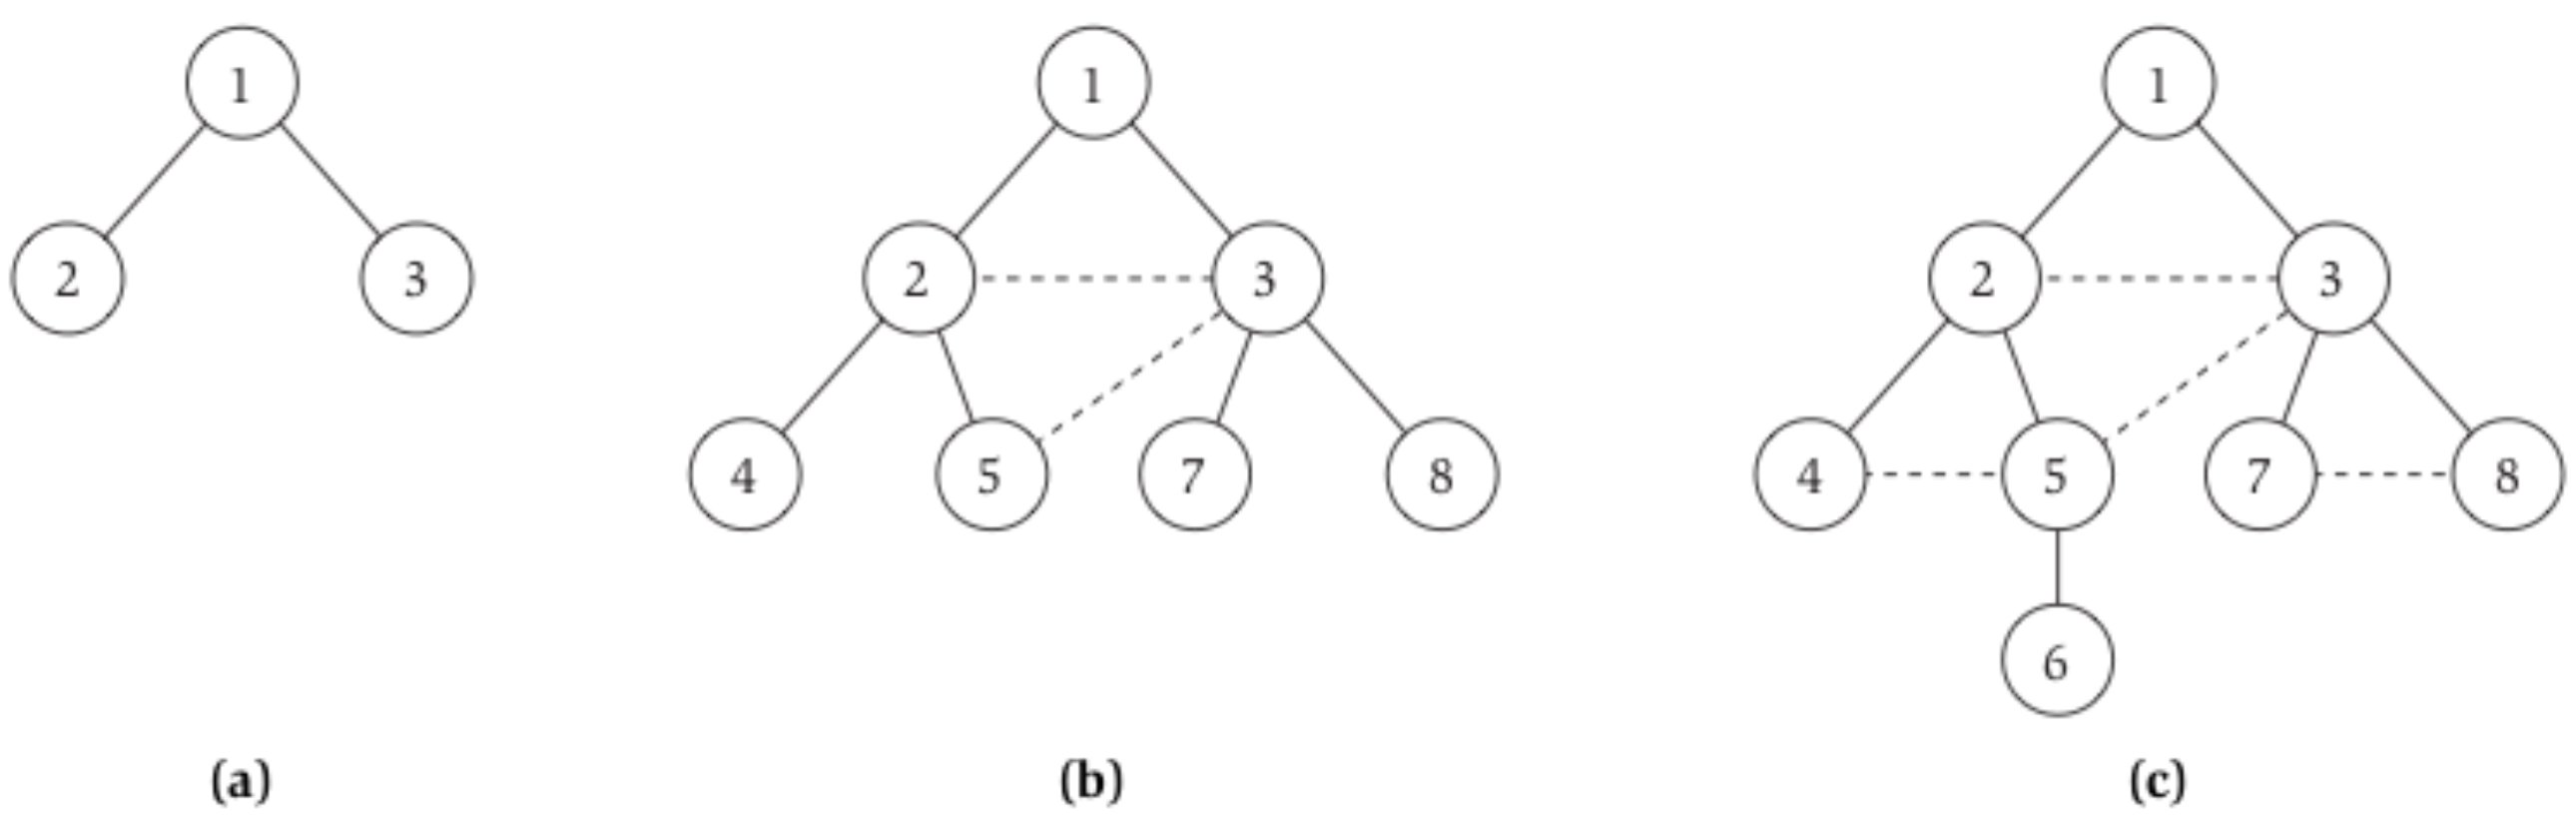
\includegraphics[width=\textwidth]{simpleGraph3}
    \caption{ The construction of a breadth-first search tree $T$ for the graph in Figure \ref{fig:simpleGraph2}, with (a), (b), and (c) depicting the successive layers that are added. The solid edges are the edges of $T$; the dotted edges are in the connected component of $G$ containing node 1, but do not belong to $T$}
\end{figure}
Figure \ref{fig:simpleGraph3} depicts the construction of a BFS tree rooted at node $1$ for the graph in Figure \ref{fig:simpleGraph2}. The solid edges are the edges of $T$; the dotted edges are edges of $G$ that do not belong to $T$. The execution of BFS that produces this tree can be described as follows.
\begin{enumerate}
\item Starting from node 1, layer $L_{1}$ consists of the nodes {2, 3}.
\item Layer $L_{2}$ is the n grown by considering the nodes in layer $L_{1}$ in order (say, first 2, then 3). Thus we discover nodes 4 and 5 as soon as we look at 2, so 2 becomes their parent. When we consider node 2, we also discover an edge to 3, but this isn't added to the BFS tree, since we already know about node 3.\par
We first discover nodes 7 and 8 when we look at node 3. On the other hand, the edge from 3 to 5 is another edge of G that does not end up in the BFS tree, because by the time we look at this edge out of node 3, we already know about node 5.
\item We then consider the nodes in layer $L_{2}$ in order, but the only new node discovered when we look through $L_{2}$  is node 6, which is added to layer $L_{3}$ . Note that the edges $(4, 5)$ and $(7, 8)$ don't get added to the BFS tree, because they don't result in the discovery of new nodes.
(d) No new nodes are discovered when node 6 is examined, so nothing is put in layer $L_{4}$, and the algorithm terminates. The full BFS tree is depicted in Figure \ref{fig:simpleGraph3}(c).
\end{enumerate}
We notice that as we ran BFS on this graph, the nontree edges all either connected nodes in the same layer, or connected nodes in adjacent layers. We now prove that this is a property of BFS trees in general.
\begin{lemma}
Let $T$ be a breadth-first search tree, let $x$ and $y$ be nodes in $T$ belonging to layers $L_{i} and L_{j}$ respectively, and let $(x, y)$ be an edge of $G$. Then $i and j$ differ by at most 1.
\end{lemma}
\textbf{Proof} Suppose by way of contradiction that $i and j$ differed by more than 1; in particular, suppose $i < j − 1$. Now consider the point in the BFS algorithm when the edges incident to $x$ were being examined. Since $x$ belongs to layer $L_{i}$, the only nodes discovered from $x$ belong to layers $L_{i+1}$ and earlier; hence, if $y$ is a neighbor of $x$, then it should have been discovered by this point at the latest and hence should belong to layer $L_{i+1}$ or earlier.
\begin{figure}[h]
    \centering
    \label{fig:simpleGraph4}
    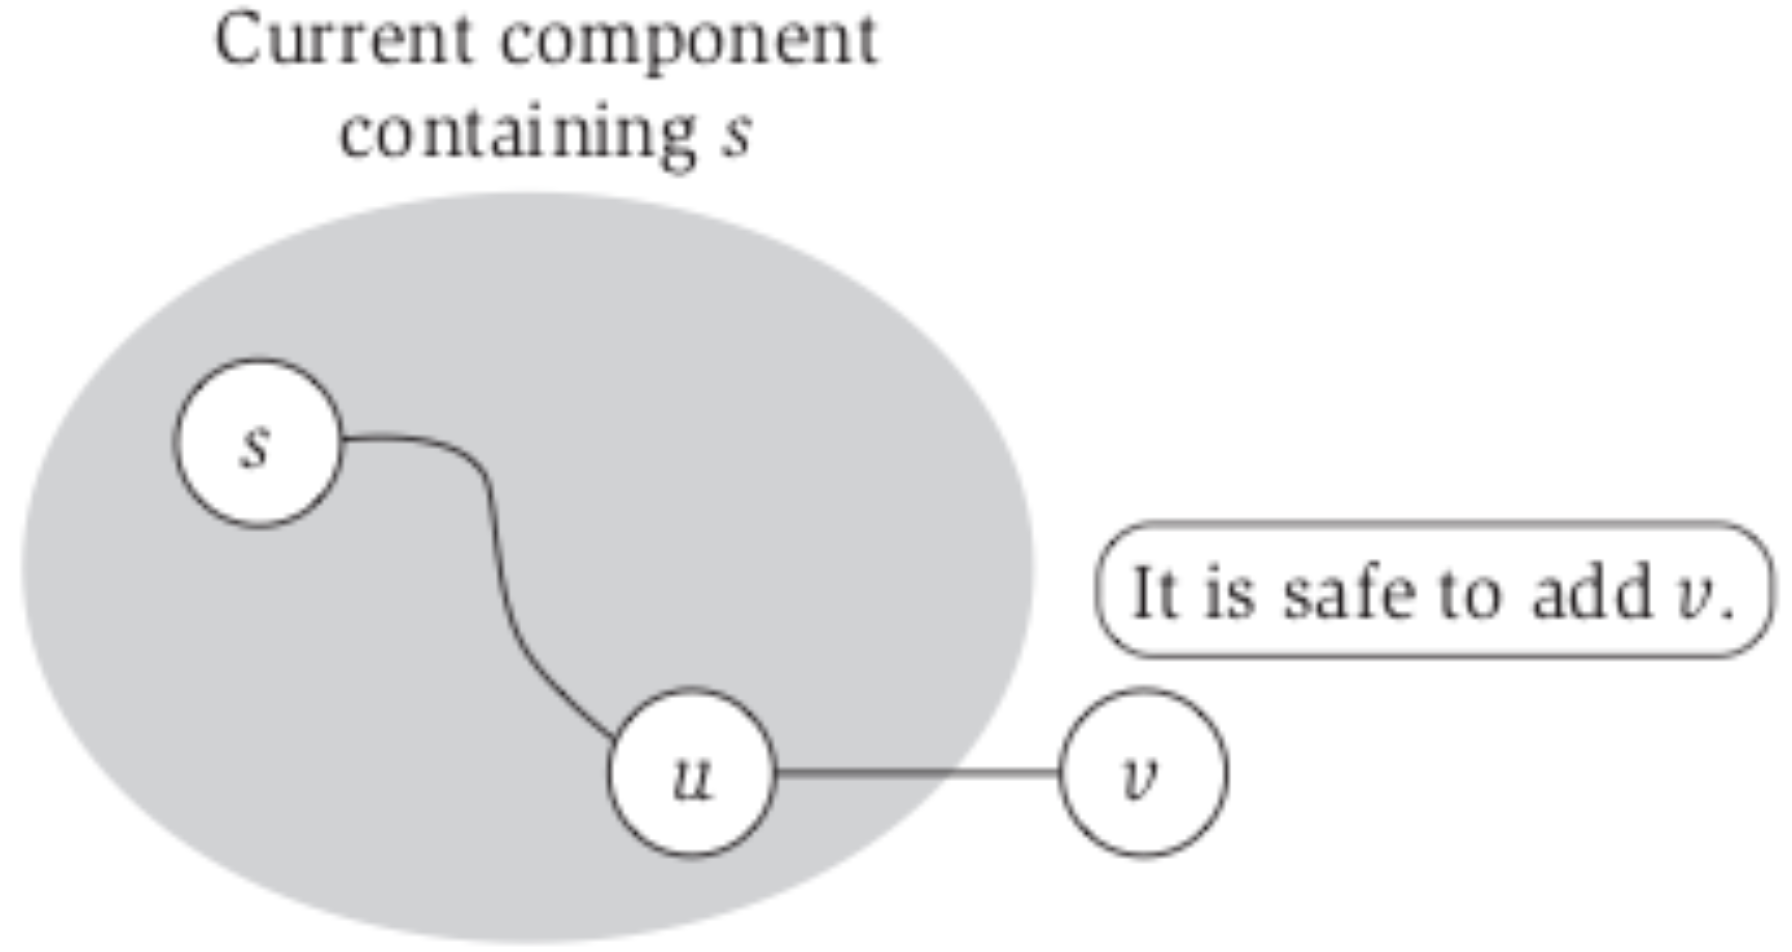
\includegraphics[width=\textwidth]{simpleGraph4}
    \caption{ When growing the connected component containing $s$, we look for nodes like $v$ that have not yet been visited.}
\end{figure}
\subsubsection{Exploring a Connected Component}
The set of nodes discovered by the BFS algorithm is precisely those reachable from the starting node $s$. We will refer to this set $R$ as the connected component of $G$ containing $s$; and once we know the \textit{connected component} containing $s$, we can simply check whether $t$ belongs to it so as to answer the question of $s-t$ connectivity.\par
Now, if one thinks about it, it's clear that BFS is just one possible way to produce this component. At a more general level, we can build the component $R$ by "exploring" $G$ in any order, starting from $s$. To start off, we define $R = \{s\}$. Then at any point in time, if we find an edge $(u, v)$ where $u \in R$ and $v \notin R$, we can add $v$ to $R$. Indeed, if there is a path $P$ from $s$ to $u$, then there is a path from $s$ to $v$ obtained by first following $P$ and then following the edge $(u, v)$. Figure \ref{fig:simpleGraph4} illustrates this basic step in growing the component $R$.\par
Suppose we continue growing the set $R$ until there are no more edges leading out of $R$; in other words, we run the following algorithm.
\begin{figure}[h]
    \centering
    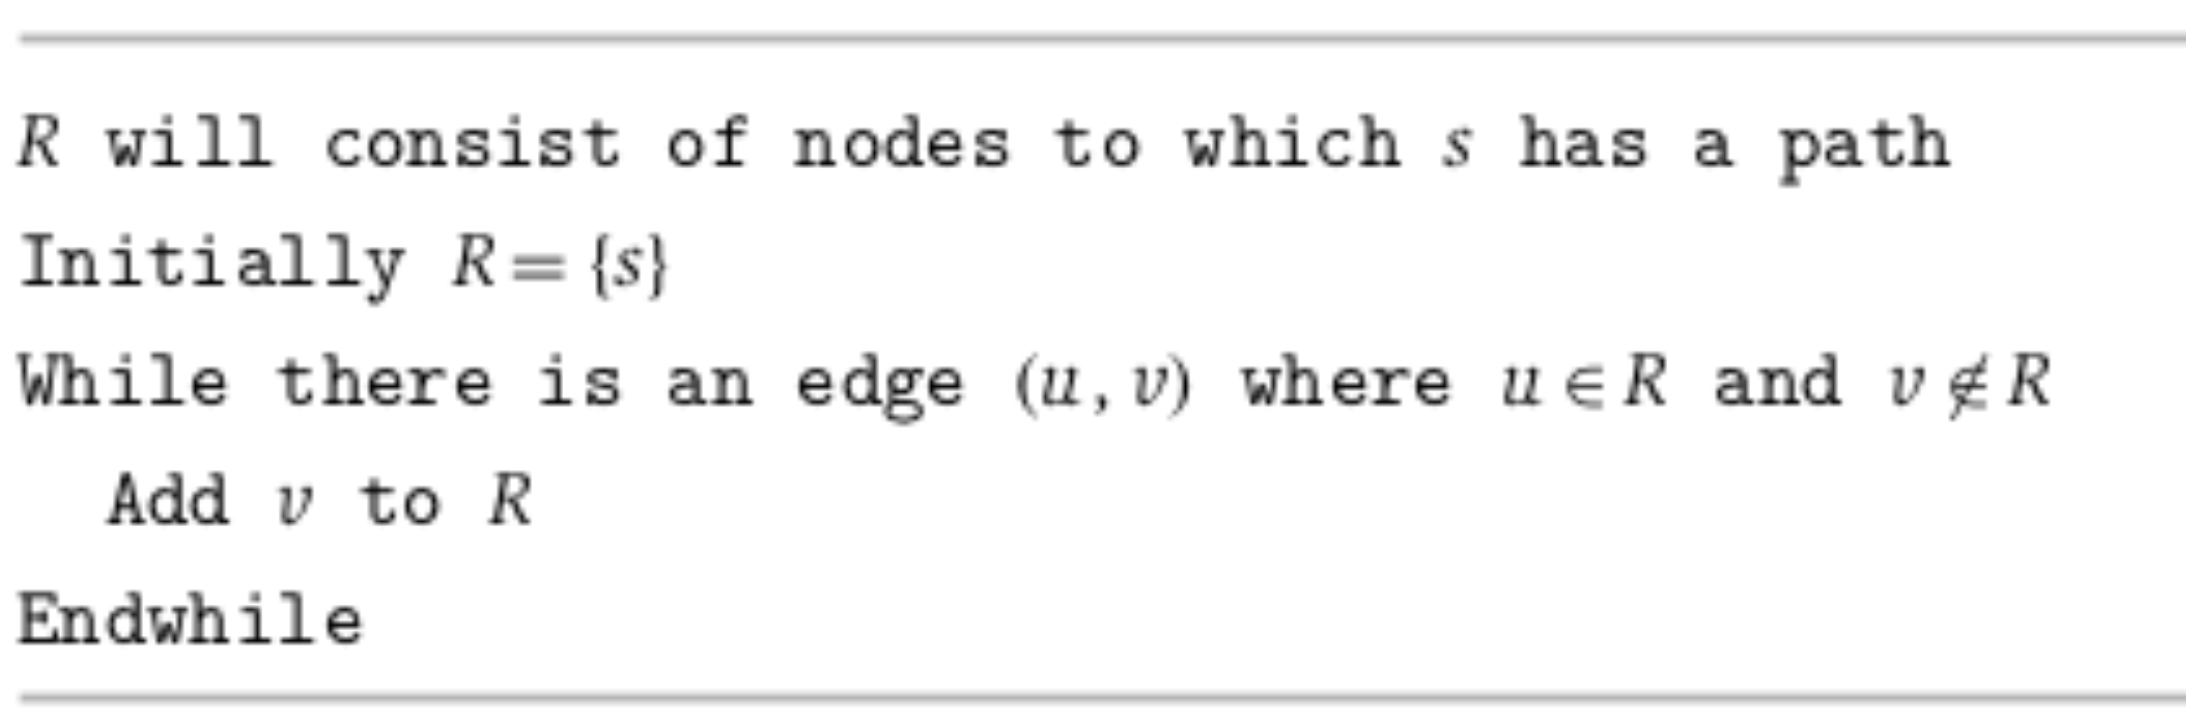
\includegraphics[width=\textwidth]{simpleGraph5}
\end{figure}
\begin{lemma}
The set $R$ produced at the end of the algorithm is precisely the connected component of $G$ containing $s$.
\end{lemma}
\textbf{Proof} We have already argued that for any node $v \in R$, there is a path from $s$ to $v$.\par
Now, consider a node $w \notin R$, and suppose by way of contradiction, that there is an $s-w$ path $P$ in $G$. Since $s \in R$ but $w \notin  R$, there must be a first node $v$ on $P$ that does not belong to $R$; and this node $v$ is not equal to $s$. Thus there is a node $u$ immediately preceding $v$ on $P$, so $(u, v)$ is an edge. Moreover, since $v$ is the first node on $P$ that does not belong to $R$, we must have $u \in R$. It follows that $(u, v)$ is an edge where $u \in R$ and $v \in R$; this contradicts the stopping rule for the algorithm.\par
For any node t in the component $R$, observe that it is easy to recover the actual path from s to t along the lines of the argument above: we simply record, for each node $v$, the edge $(u, v)$ that was considered in the iteration in which $v$ was added to $R$. Then, by tracing these edges backward from $t$, we proceed through a sequence of nodes that were added in earlier and earlier iterations, eventually reaching s; this defines an $s-t$ path.\par
To conclude, we notice that the general algorithm we have defined to grow $R$ is underspecified, so how do we decide which edge to consider next? The BFS algorithm arises, in particular, as a particular way of ordering the nodes we visit - in successive layers, based on their distance from $s$. But there are other natural ways to grow the component, several of which lead to efficient algorithms for the connectivity problem while producing search patterns with different structures. We now go on to discuss a different one of these algorithms, \textit{depth-first search}, and develop some of its basic properties.
\subsection{Depth First Search (DFS)}
Another natural method to find the nodes reachable from s is the approach you might take if the graph $G$ were truly a maze of interconnected rooms and you were walking around in it. You'd start from s and try the first edge leading out of it, to a node $v$. You'd then follow the first edge leading out of v, and continue in this way until you reached a "dead end" - a node for which you had already explored all its neighbors. You'd then backtrack until you got to a node with an unexplored neighbor, and resume from there. We call this algorithm depth - first search (DFS), since it explores G by going as deeply as possible and only retreating when necessary.\par
DFS is also a particular implementation of the generic component-growing algorithm that we introduced earlier. It is most easily described in recursive form: we can invoke DFS from any starting point but maintain global knowledge of which nodes have already been explored.\par
\begin{figure}[h]
    \centering
    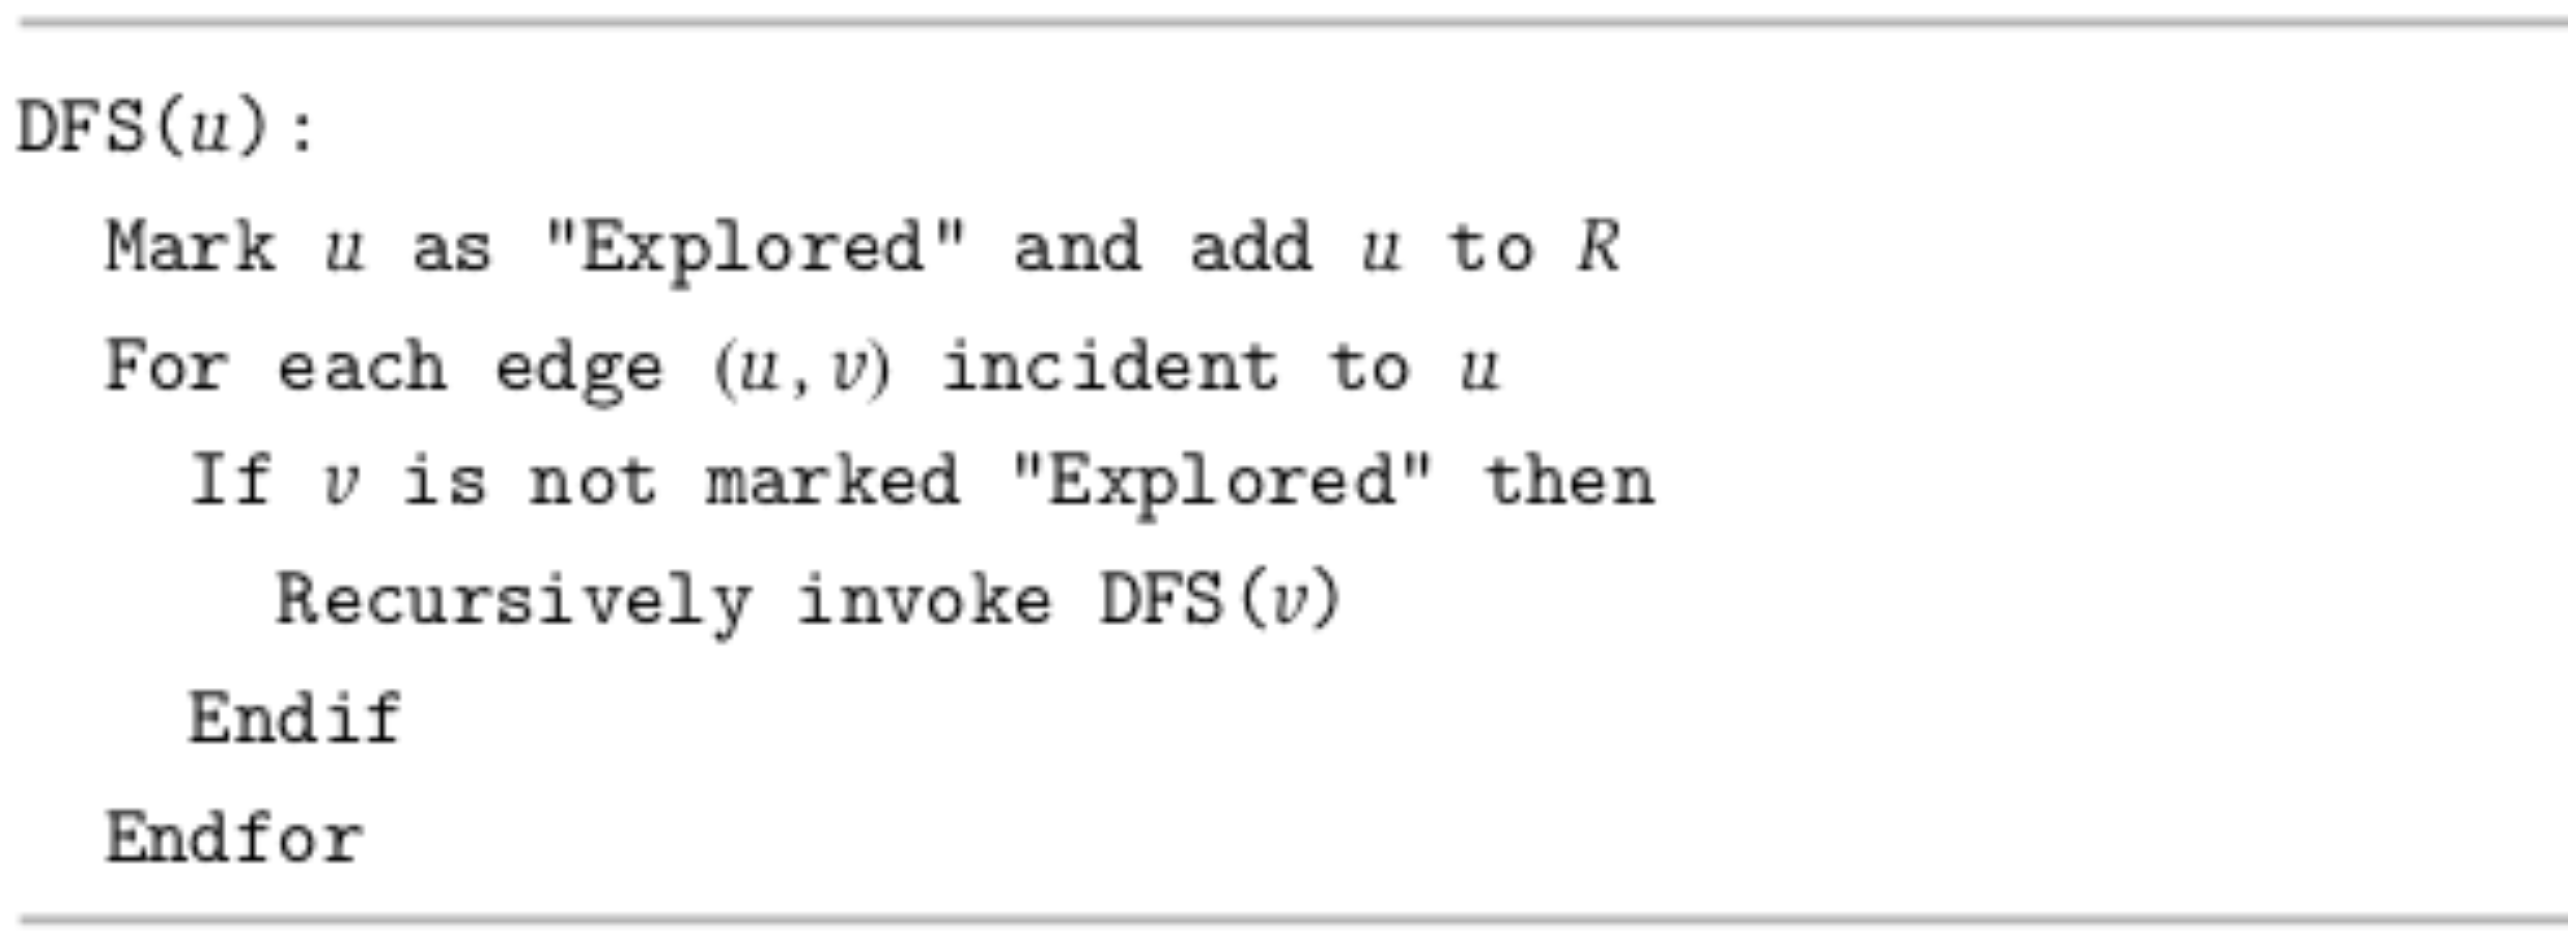
\includegraphics[width=\textwidth]{simpleGraph6}
\end{figure}
To apply this to $s-t$ connectivity, we simply declare all nodes initially to be not explored, and invoke DFS(s).
\begin{figure}[h]
    \centering
    \label{fig:simpleGraph7}
    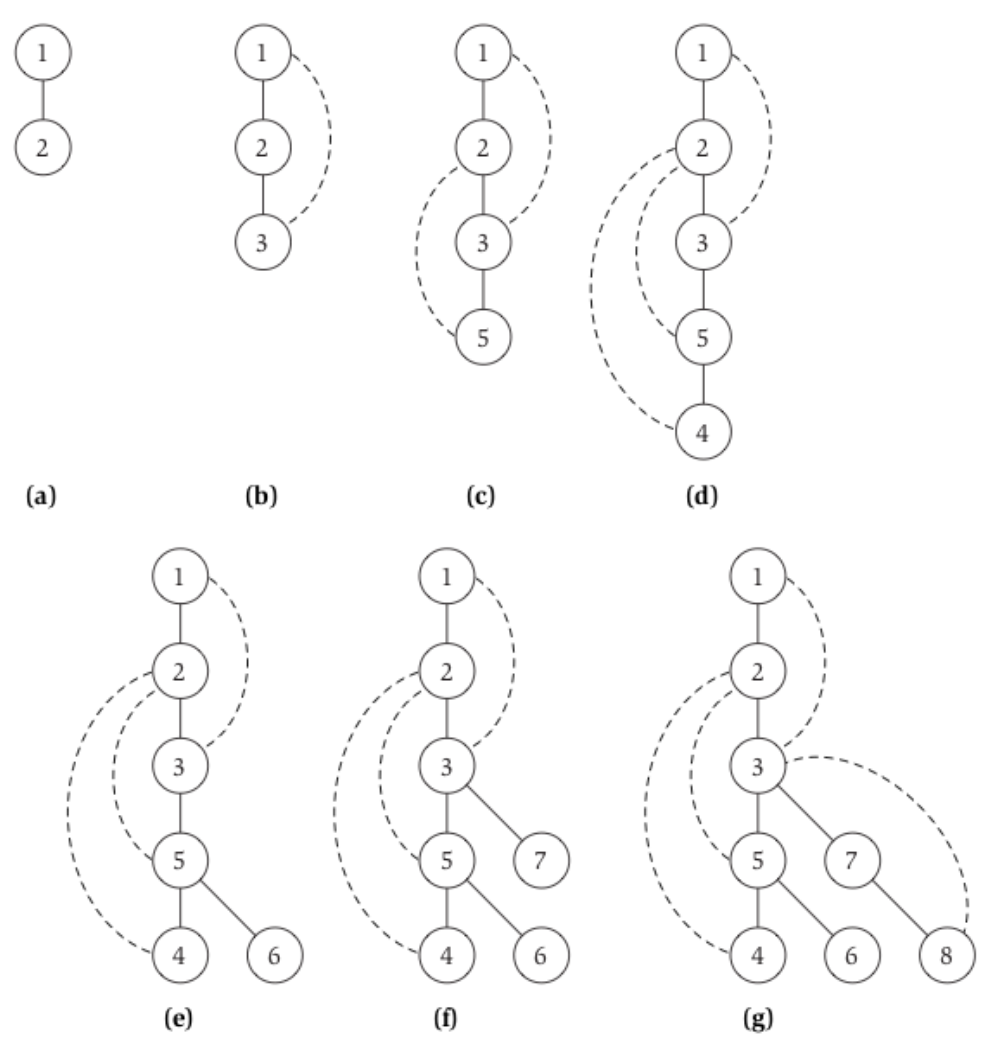
\includegraphics[width=\textwidth]{simpleGraph7}
    \caption{ The construction of a depth-first search tree $T$ for the graph in Figure \ref{fig:simpleGraph2}, with (a) through (g) depicting the nodes as they are discovered in sequence. The solid edges are the edges of $T$; the dotted edges are edges of $G$ that do not belong to $T$.}
\end{figure}
There are some fundamental similarities and some fundamental differences between DFS and BFS. The similarities are based on the fact that they both build the connected component containing $s$, and we will see in the next section that they achieve qualitatively similar levels of efficiency.\par
While DFS ultimately visits exactly the same set of nodes as BFS, it typically does so in a very different order; it probes its way down long paths, potentially getting very far from $s$, before backing up to try nearer unexplored nodes. We can see a reflection of this difference in the fact that, like BFS, the DFS algorithm yields a natural rooted tree T on the component containing $s$, but the tree will generally have a very different structure. We make $s$ the root of the tree $T$, and make $u$ the parent of $v$ when $u$ is responsible for the discovery of $v$. That is, whenever $DFS(v)$ is invoked directly during the call to $DFS(u)$, we add the edge $(u, v)$ to $T$. The resulting tree is called a depth-first search tree of the component $R$.\par
Figure \ref{fig:simpleGraph7} depicts the construction of a DFS tree rooted at node 1 for the graph in Figure \ref{fig:simpleGraph2}. The solid edges are the edges of $T$; the dotted edges are edges of $G$ that do not belong to $T$. The execution of DFS begins by building a path on nodes $1, 2, 3, 5, 4$. The execution reaches a dead end at 4, since there are no new nodes to find, and so it "backs up" to 5, finds node 6, backs up again to 3, and finds nodes 7 and 8. At this point there are no new nodes to find in the connected component, so all the pending recursive DFS calls terminate, one by one, and the execution comes to an end. The full DFS tree is depicted in Figure \ref{fig:simpleGraph7}(g).\par
This example suggests the characteristic way in which DFS trees look different from BFS trees. Rather than having root-to-leaf paths that are as short as possible, they tend to be quite narrow and deep. However, as in the case of BFS, we can say something quite strong about the way in which non-tree edges of $G$ must be arranged relative to the edges of a DFS tree $T$: as in the figure, non-tree edges can only connect ancestors of $T$ to descendants.\par
To establish this, we first observe the following property of the DFS algorithm and the tree that it produces.
\begin{lemma}[a]
For a given recursive call $DFS(u)$, all nodes that are marked "Explored" between the invocation and end of this recursive call are descendants of $u$ in $T$.
\end{lemma}
Using this we prove 
\begin{lemma}
Let $T$ be a depth-first search tree, let $x$ and $y$ be nodes in $T$, and let $(x, y)$ be an edge of $G$ that is not an edge of $T$. Then one of $x$ or $y$ is an ancestor of the other.\par
\textbf{Proof}. Suppose that $(x,y)$ is an edge of $G$ that is not an edge of T,and suppose without loss of generality that $x$ is reached first by the DFS algorithm. When the edge $(x, y)$ is examined during the execution of $DFS(x)$, it is not added to $T$ because $y$ is marked "Explored". Since $y$ was not marked "Explored" when $DFS(x)$ was first invoked, it is a node that was discovered between the invocation and end of the recursive call $DFS(x)$. It follows from  above that $y$ is a descendant of $x$.
\end{lemma}
\subsubsection{The Set of All Connected Components}
So far we have been talking about the connected component containing a particular node $s$. But there is a connected component associated with each node in the graph. What is the relationship between these components?\par
In fact, this relationship is highly structured and is expressed in the following claim.\par
\begin{lemma}
For any two nodes s and t in a graph, their connected components are either identical or disjoint.
\end{lemma}
This is a statement that is very clear intuitively, if one looks at a graph like the example in Figure \ref{fig:simpleGraph2}. The graph is divided into multiple pieces with no edges between them; the largest piece is the connected component of nodes 1 through 8, the medium piece is the connected component of nodes 11, 12, and 13, and the smallest piece is the connected component of nodes 9 and 10. To prove the statement in general, we just need to show how to define these "pieces" precisely for an arbitrary graph.\par
\textbf{Proof}. Consider any two nodes $s$ and $t$ in a graph $G$ with the property that there is a path between $s$ and $t$. We claim that the connected components containing $s$ and $t$ are the same set. Indeed, for any node $v$ in the component of $s$, the node $v$ must also be reachable from $t$ by a path: we can just walk from $t$ to $s$, and then on from $s$ to $v$. The same reasoning works with the roles of $s$ and $t$ reversed, and so a node is in the component of one if and only if it is in the component of the other.\par
On the other hand, if there is no path between $s$ and $t$, then there cannot be a node $v$ that is in the connected component of each. For if there were such a node $v$, then we could walk from $s$ to $v$ and then on to $t$, constructing a path between $s$ and $t$. Thus, if there is no path between $s$ and $t$, then their connected components are disjoint.\par
This proof suggests a natural algorithm for producing all the connected components of a graph, by growing them one component at a time. We start with an arbitrary node $s$, and we use BFS (or DFS) to generate its connected component. We then find a node $v$ (if any) that was not visited by the search from $s$, and iterate, using BFS starting from $v$, to generate its connected component-which will be disjoint from the component of $s$. We continue in this way until al	l nodes have been visited.
\section{Implementation}
dsdkgj dgkdsfjgsdf hjgbhdsf dsdkgj dgkdsfjgsdf hjgbhdsf bghjsbfg jiojoin sdiufg moerijndfsgo kmslfgoi irntsz asif eknd knr ksagnabghjsbfg jiojoin sdiufg moerijndfsgo kmslfgoi irntsz asif eknd knr ksagna dsdkgj dgkdsfjgsdf hjgbhdsf bghjsbfg jiojoin sdiufg moerijndfsgo kmslfgoi irntsz asif eknd knr ksagna
\section{Sample Application}
\section{Exercises}
\begin{enumerate}
\item Given an adjacency-list representation of a directed graph, how long does it take to compute the out-degree of every vertex? How long does it take to compute the in-degrees?
\item Give an adjacency-list representation for a complete binary tree on 7 vertices. Give an equivalent adjacency-matrix representation. Assume that vertices are numbered from 1 to 7 as in a binary heap.
\end{enumerate}
\part{Algorithm Design}
\chapter{Divide and Conquer}
\chapter{Dynamic Programming}
\chapter{Greedy Algorithms}
\part{Additional Topics}
\chapter{String Matching}
\chapter{Multithreaded Algorithms}
\chapter{Matrix Operations}
\chapter{NP-Completeness}
\end{document}
